\documentclass[norsk,a4paper,12pt]{article}
\usepackage{booktabs}  % Tabs
\usepackage{graphicx}  % Pictures/figures
\usepackage{listings}  % Source code
\usepackage{color}     % Colors
\usepackage{mdframed}  % Frames
\usepackage{float}
\usepackage{hyperref}
\usepackage{subcaption}

\begin{document}
\begin{center}

\includegraphics[width=0.15\textwidth]{uio.png}\par\vspace{1cm}
{\scshape\LARGE FYS2280 - Romteknologi \par}
\vspace{0.5cm}
{\scshape\large CaNoRock XIII\par}
\vspace{1cm}
{\Large\itshape Even Marius Nordhagen\par}
\vspace{0.5cm}
{\large \today\par}
\end{center}
\section*{Introduksjon}
Vi var fem spente studenter som reiste til And{\o}ya s{\o}ndag 2. oktober for {\aa} delta p{\aa} CaNoRock 13, som er et rakettkurs med studenter fra forskjellige steder i Norge og Canada. Reisen til rakettbasen And{\o}ya Space Center (ASC) gikk ikke helt feilfritt, og p{\aa} grunn av forsinkelser fikk vi p{\aa} et tidspunkt beskjed om {\aa} belage oss p{\aa} {\aa} overnatte i Bod{\o} (hvor vi mellomlandet). Dette ble senere forandret ettersom flyet som skulle ta oss til And{\o}ya ventet, og jeg fikk oppleve den korteste mellomlandingen jeg noensinne har v{\ae}rt med p{\aa}. Siste delen av turen ble tilbakelagt med et propellfly av typen Bombardier Dash 8, som gjorde at vi omsider kom frem til ASC. Alle fotografiene i denne rapporten er tatt av meg med mindre noe annet er oppgitt. Disse er {\aa} finne i mappen \url{https://1drv.ms/f/s!At6zdGzzRAgTmJMpN5I3-rHGV6RZuQ}.
\begin{figure}[H]
\centering
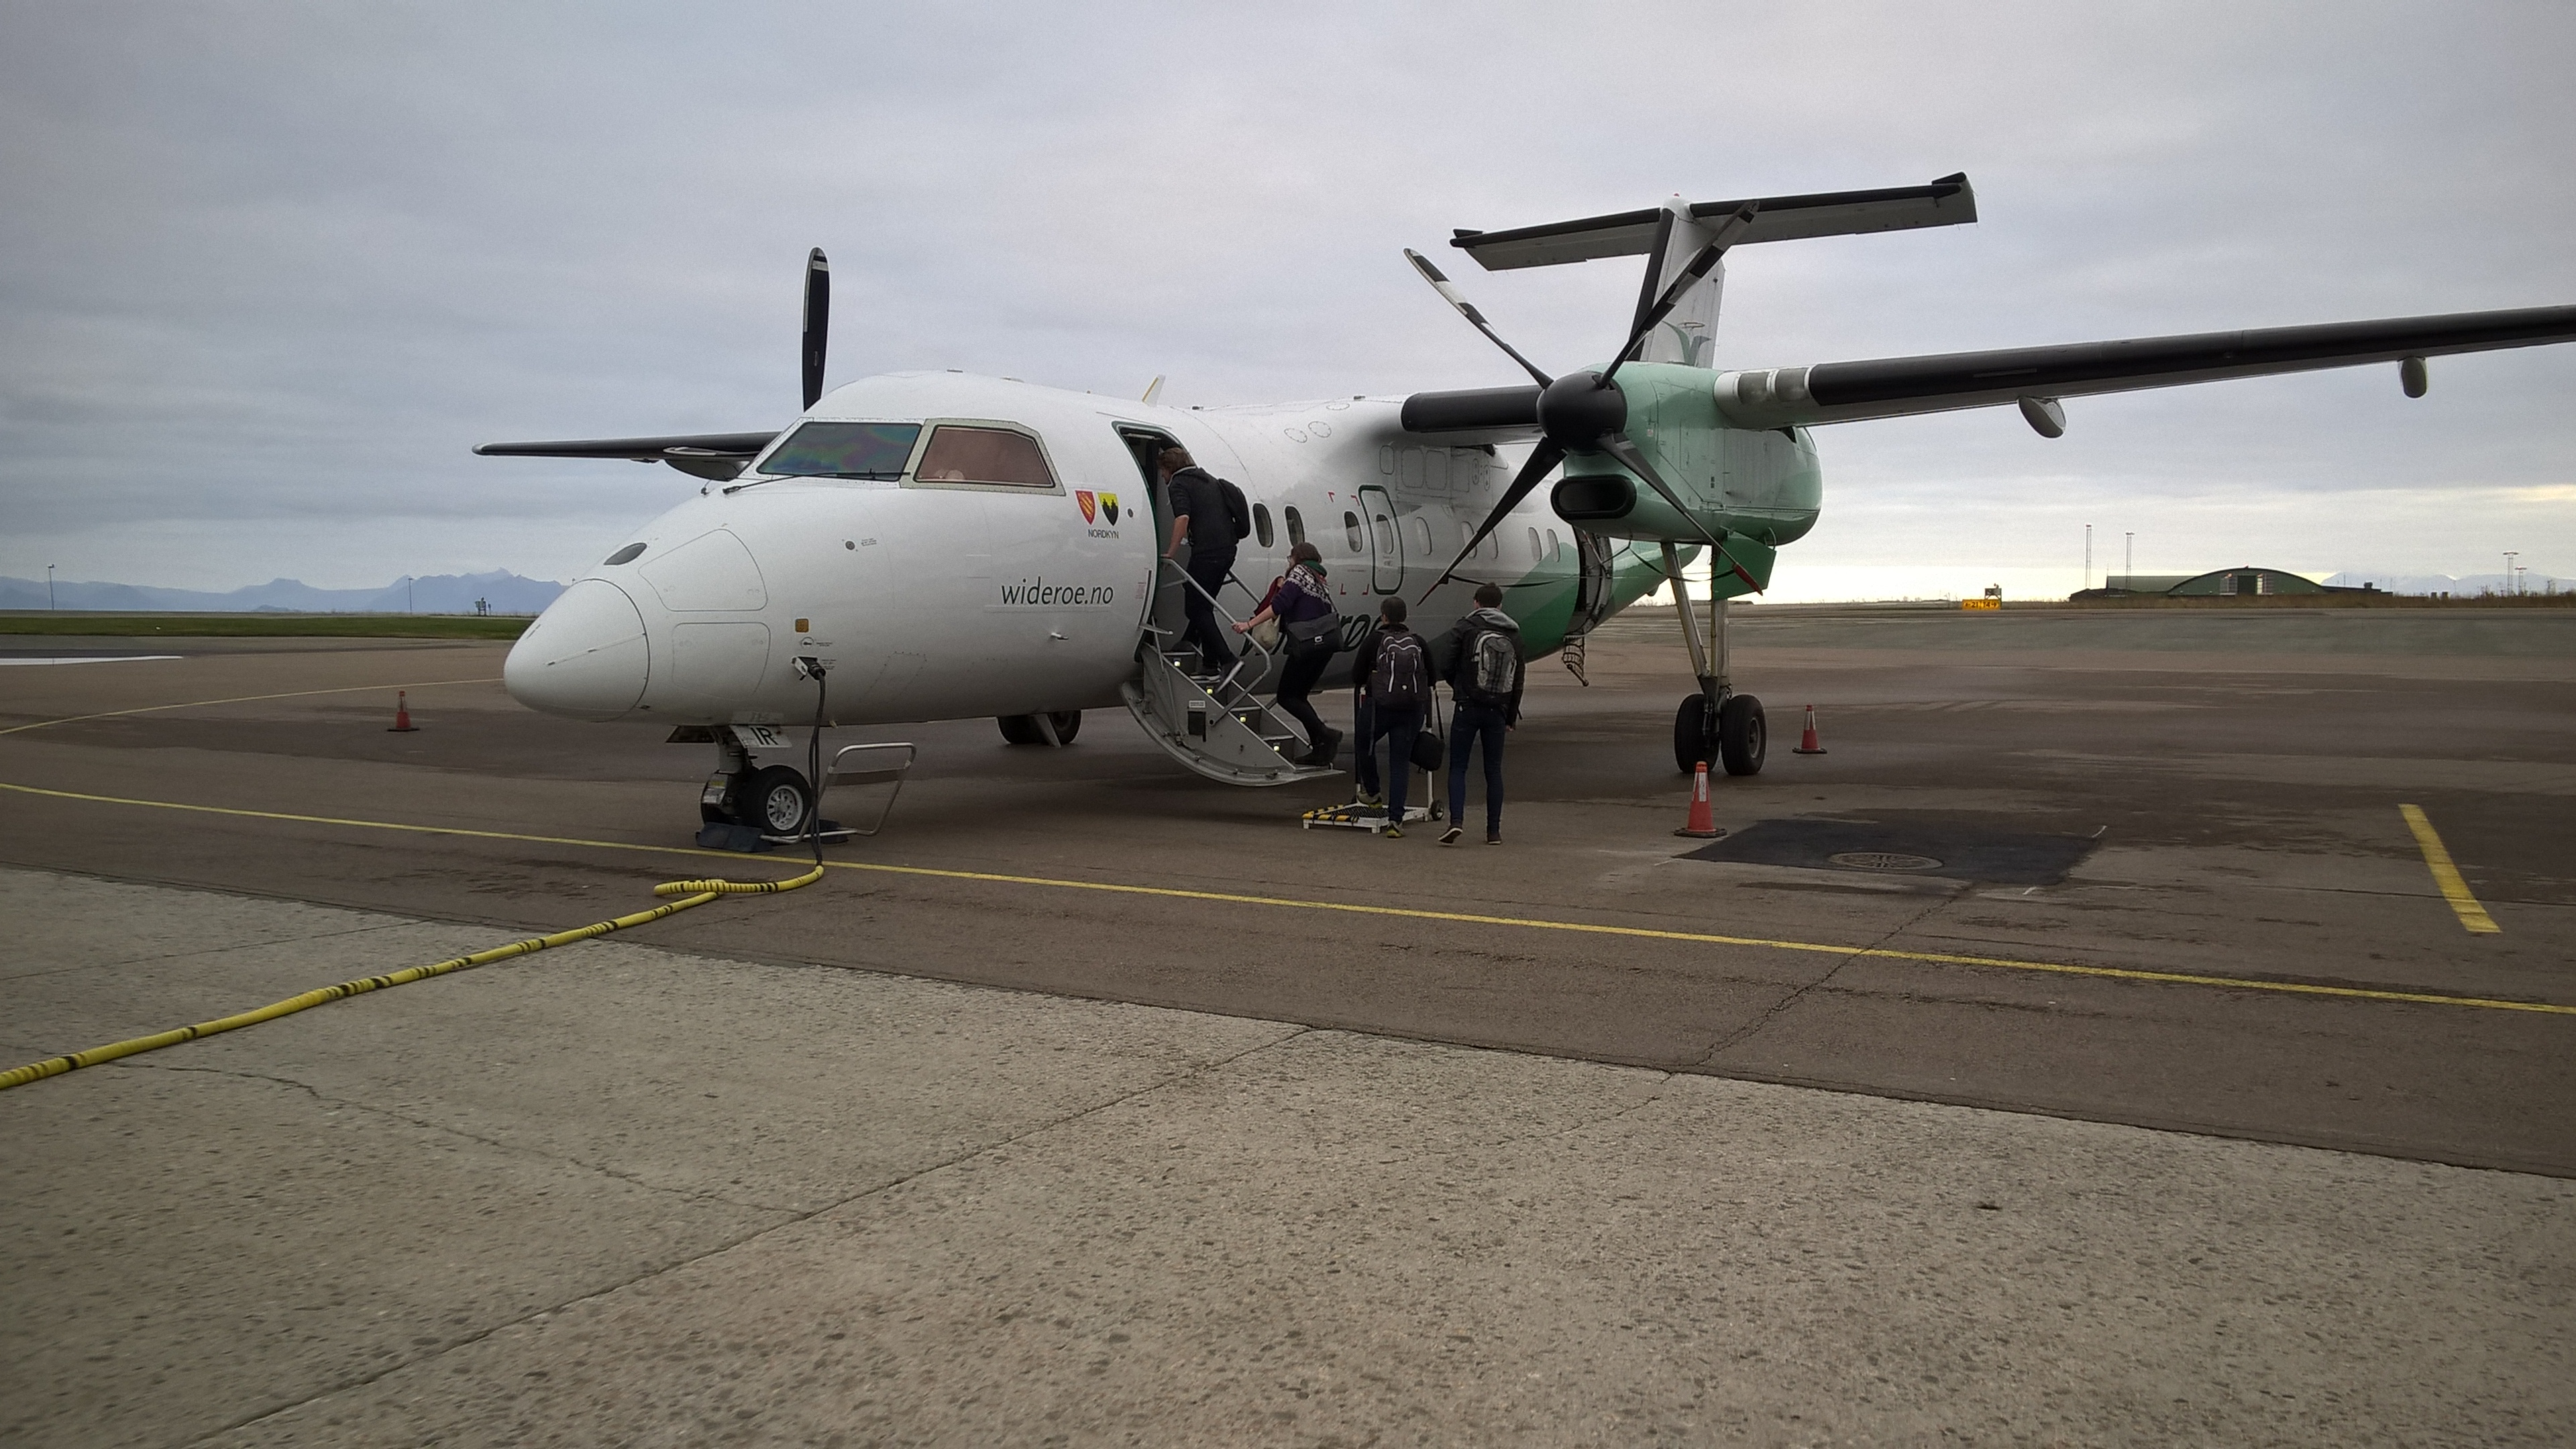
\includegraphics[width=90mm]{WP_20161007_16_11_05_Pro.jpg}
\caption{Bombardier Dash 8. Bilde tatt p{\aa} Andenes flyplass. \label{overflow}}
\end{figure}

\section*{Dag 1 - Mandag 3/10}
Den f{\o}rste dagen fikk for det meste med til {\aa} h{\o}re p{\aa} forelesninger. F{\o}rst fikk vi litt praktisk informasjon hvor vi ble presentert for fem forskjellige problemstillinger n{\aa}r det kom til raketten vi skulle v{\ae}re med {\aa} skyte opp, og vi fikk sette opp en prioriteringsliste basert p{\aa} hvilken problemstilling vi syntes var mest interessant. Deretter fungte et par korte popul{\ae}rvitenskapelige forelesninger om hvordan vi kan fjernm{\aa}le Jorda fra en satelitt, og hvordan nordlys fungerer i praksis. Til slutt fikk vi en innf{\o}ring i rakettfysikk, noe som kom godt med senere n{\aa}r vi skulle studerer raketter p{\aa} ekte, f{\o}r vi fikk vite hvilken gruppe hver av oss kom med p{\aa}. De fem gruppene var:
\begin{itemize}
\item Gruppe A: Rakettutforming
\item Gruppe B: Elektronikk
\item Gruppe C: Nyttelast
\item Gruppe D: Telegrafi
\item Gruppe E: Fysikk
\end{itemize}
Jeg var heldig og fikk v{\ae}re med p{\aa} f{\o}rstevalget mitt, Gruppe E: Fysikk, noe jeg var veldig f{\o}rn{\o}yd med. Vi ble ogs{\aa} satt til {\aa} lage hver v{\aa}r papprakett som skulle skytes opp ved hjelp av trykkluft.\par\vspace{3mm} Senere p{\aa} kvelden var det noen sosiale aktiviteter, som for det meste gikk ut p{\aa} {\aa} sitte og snakke sammen, mens vi ble servert {\o}l og brus av vertskapet.

\begin{figure}[H]
\centering
\includegraphics[width=90mm]{paperrocket.jpg}
\caption{Pappraketten til meg og Dorthea Gjestvang ble kun sl{\aa}tt av {\'e}n annen rakett. \label{overflow}}
\end{figure}

\section*{Dag 2 - Tirsdag 4/10}
Tirsdagen startet med at vi dro p{\aa} to fiktive romferder med Spaceship Aurora, hvor halvparten satt i romskipet under den f{\o}rste ferden, mens resten passet p{\aa} at alt gikk som det skulle. Deretter byttet vi roller til neste ferd (ettersom man ikke kan v{\ae}re i rommet for lenge av gangen). \par\vspace{3mm}
Deretter gikk vi igang med gruppejobbingen, hvor vi som fysikkgruppe hadde ansvaret for {\aa} bearbeide dataene som vi fikk fra telegrafigruppen og sammenligne disse med beregnede resultater. Elektronikkgruppen laget de elektriske apparatene (sensorene) til raketten, som besto av et akselerometer, en temperatursensor, en trykksensor og et magnetometer. De beregnede resultatene fikk vi fra en rakettsimulering, og i tillegg skulle gruppen jeg var p{\aa} sende opp en v{\ae}rballong. Det f{\o}rste vi gjorde var {\aa} starte simuleringen, hvor vi fikk et anslag av hvor h{\o}y temperatur og trykk vi vil f{\aa} under take-off av raketten. Vi m{\aa}tte starte denne raskest mulig fordi simueringen tok veldig lang tid. \par\vspace{3mm}
Det neste p{\aa} agendaen var en forelesning om v{\ae}rballonger, hvor vi l{\ae}rte det mest grunnleggende om disse ballongene. Dette kom veldig godt med n{\aa}r vi etter forelesningen skulle launche en slik ballong. V{\ae}rballongen vi skulle launche ble utstyrt med en enkelt komponent som bestod av en GPS-sensor som bestemte posisjon i tre dimensjoner, samt en temperatursensor og en fuktighetsm{\aa}ler. Tanken var at ballongen ble f{\o}rt av vinden, s{\aa} vi kunne bestemme vinden ut fra hvordan ballongen beveget seg. Vi hadde ingen trykksensor, men beregnet trykk ut ifra en trykkmodell som var basert p{\aa} h{\o}yde (posisjon i z-retning). Vi fylte ballongen med Helium (Hydrogen hadde v{\ae}rt bedre siden det er lettere, men p{\aa} grunn av sikkerhet m{\aa}tte vi ta til takke med Helium), festet m{\aa}leapparatet og slapp den. Vi fikk vite at ballongen ville doble siden radius f{\o}r den ville briste, noe som vil si at den hadde radius p{\aa} ca. 4.5 meter p{\aa} det meste. De faktiske dataene fra ballongen m{\aa}tte vi vente p{\aa} til dagen etter. Etter launchingen gikk vi tilbake til klasserommet, hvor vi begynte {\aa} lage modellraketter basert p{\aa} bruksanvisninger.

\begin{figure}[H]
\centering
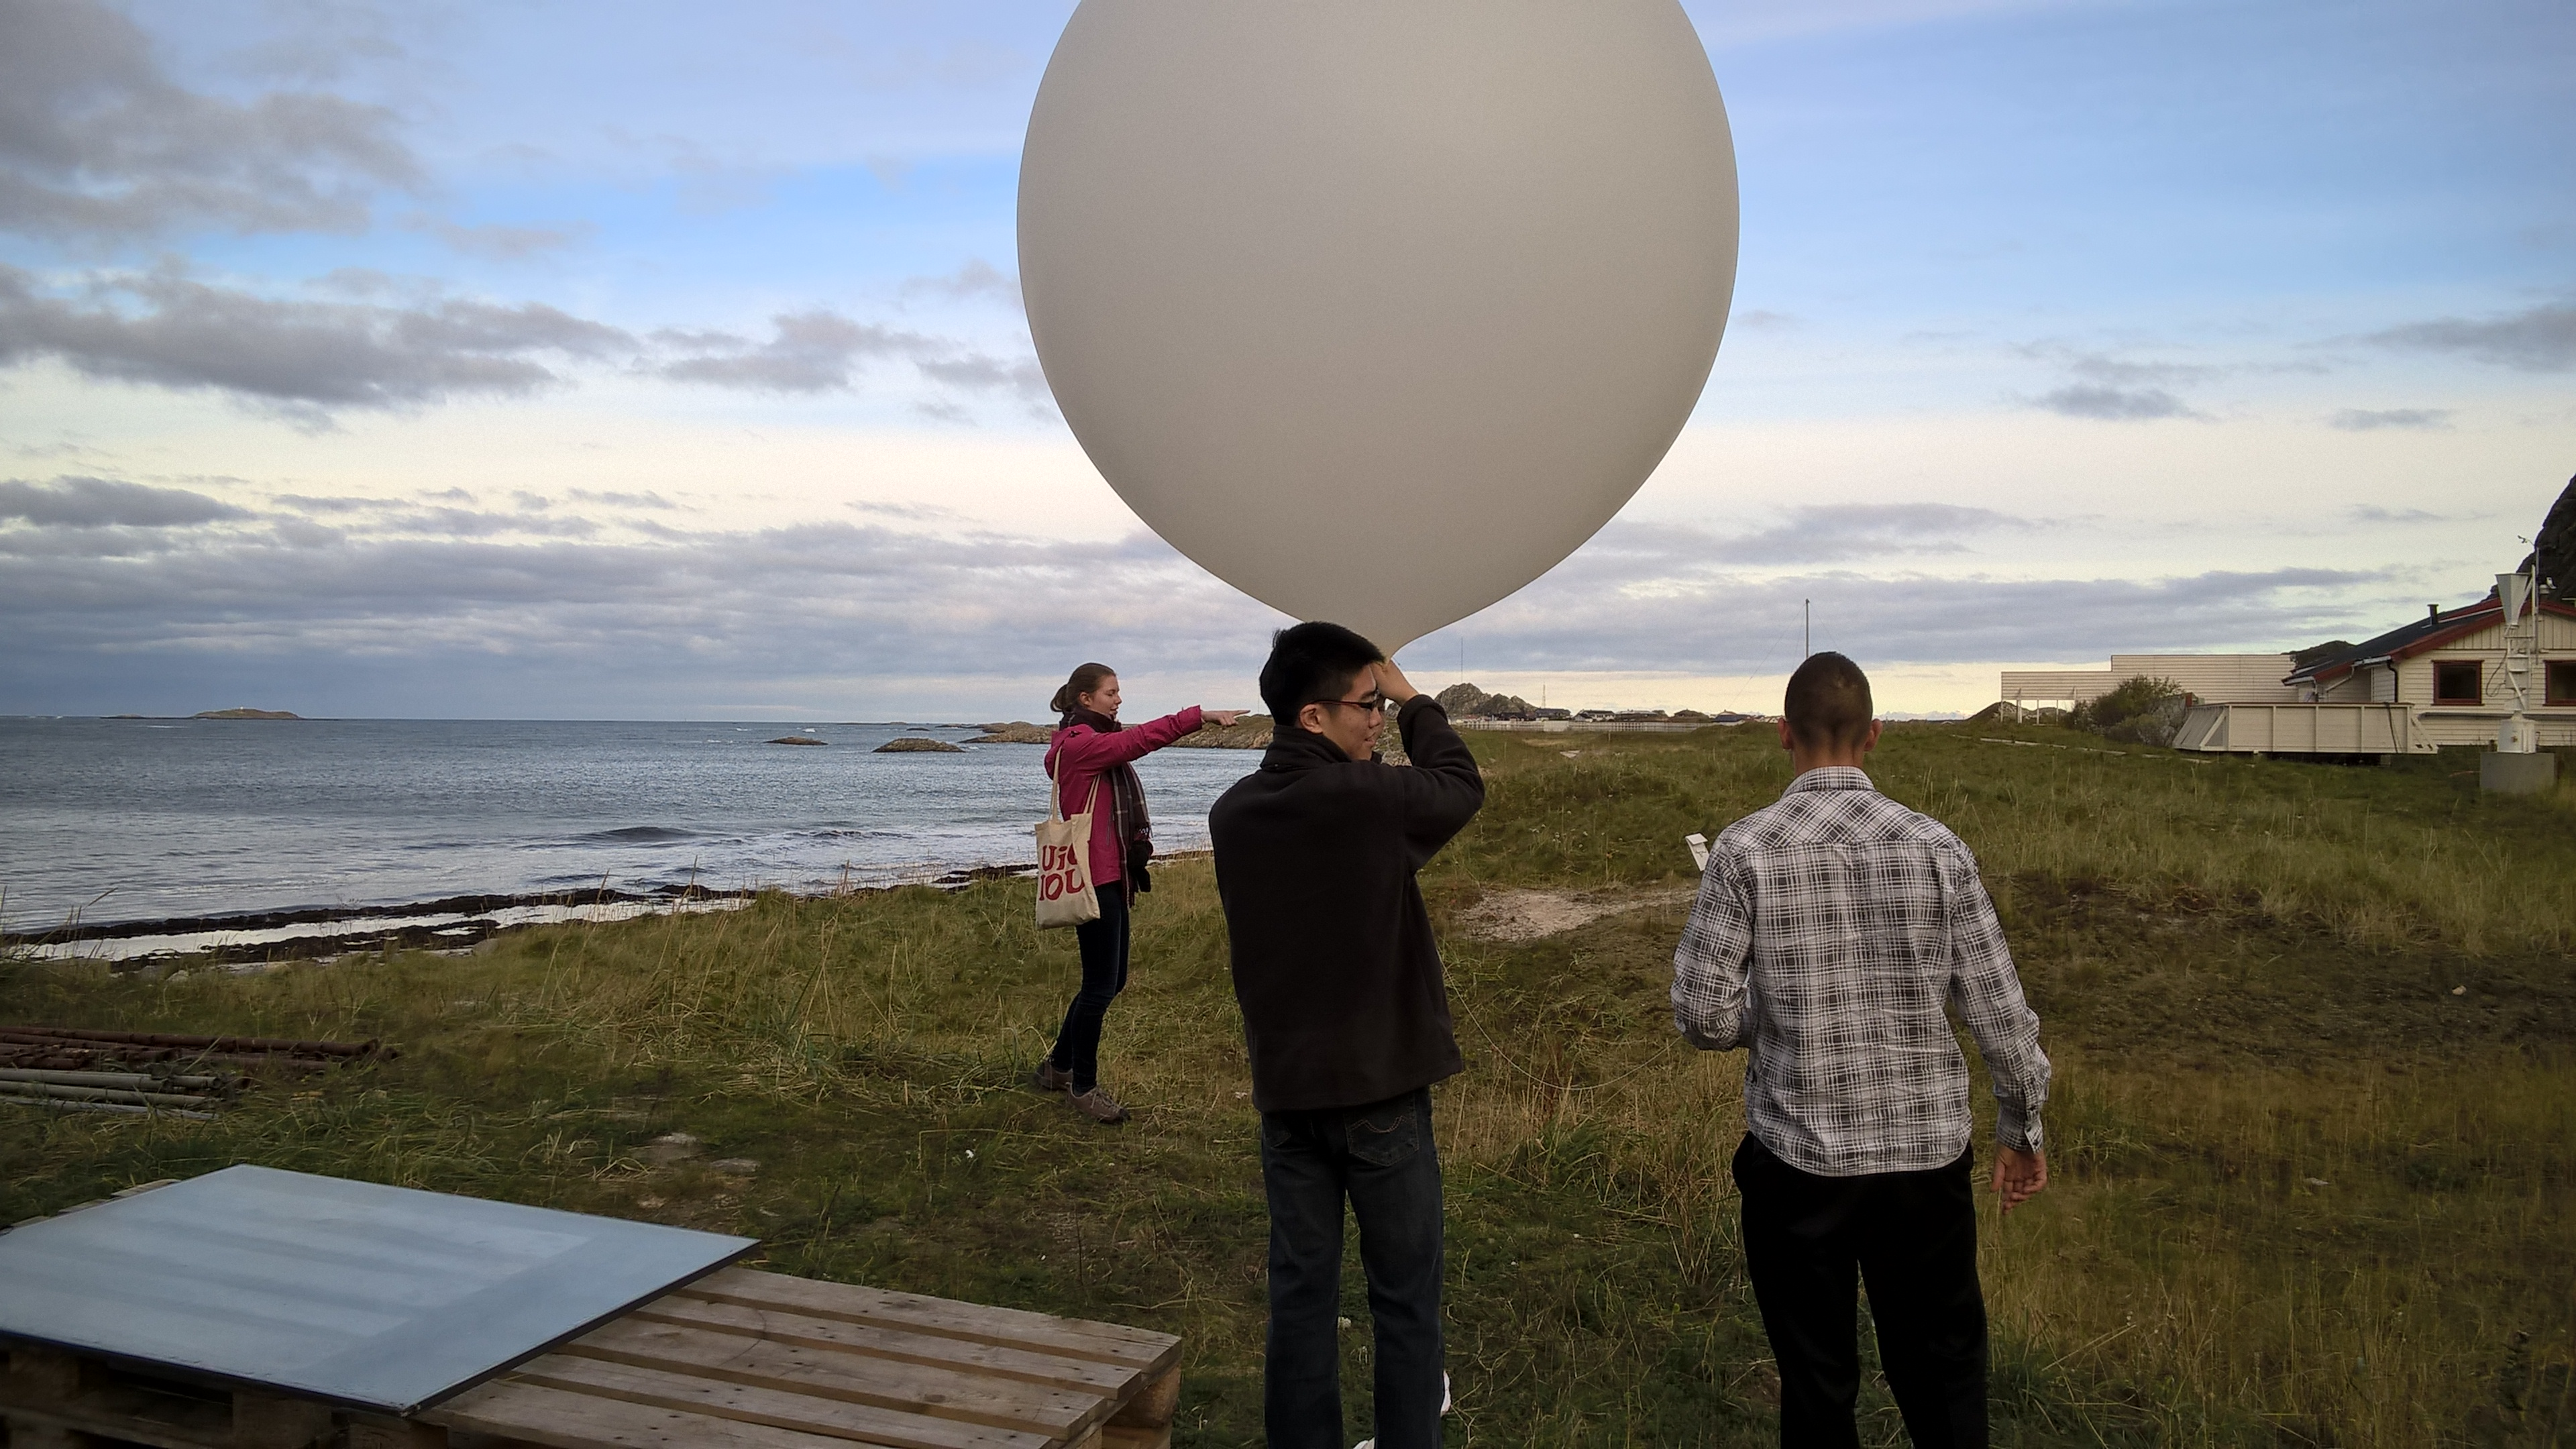
\includegraphics[width=90mm]{balloon.jpg}
\caption{Bilde tatt like f{\o}r vi skulle launche ballongen. Fra venstre: Dorthea Gjestvang, Henry Su og David Bellerose. \label{overflow}}
\end{figure}
Deretter var det omvisning rundt p{\aa} ASC, hvor vi fik se stedet hvor de setter sammen rakettene, utskytningsrampene, og de forskjellige konstrollsenterene. Utp{\aa} kvelden reiste vi til Andenes hvor vi spiste pizza, drakk {\o}l og hadde det hyggelig. Da vi kom ut fra restauranten, var det nordlys p{\aa} himmelen, noe som er en opplevelse for en "s{\o}ring". 
\begin{figure}[H]
\centering
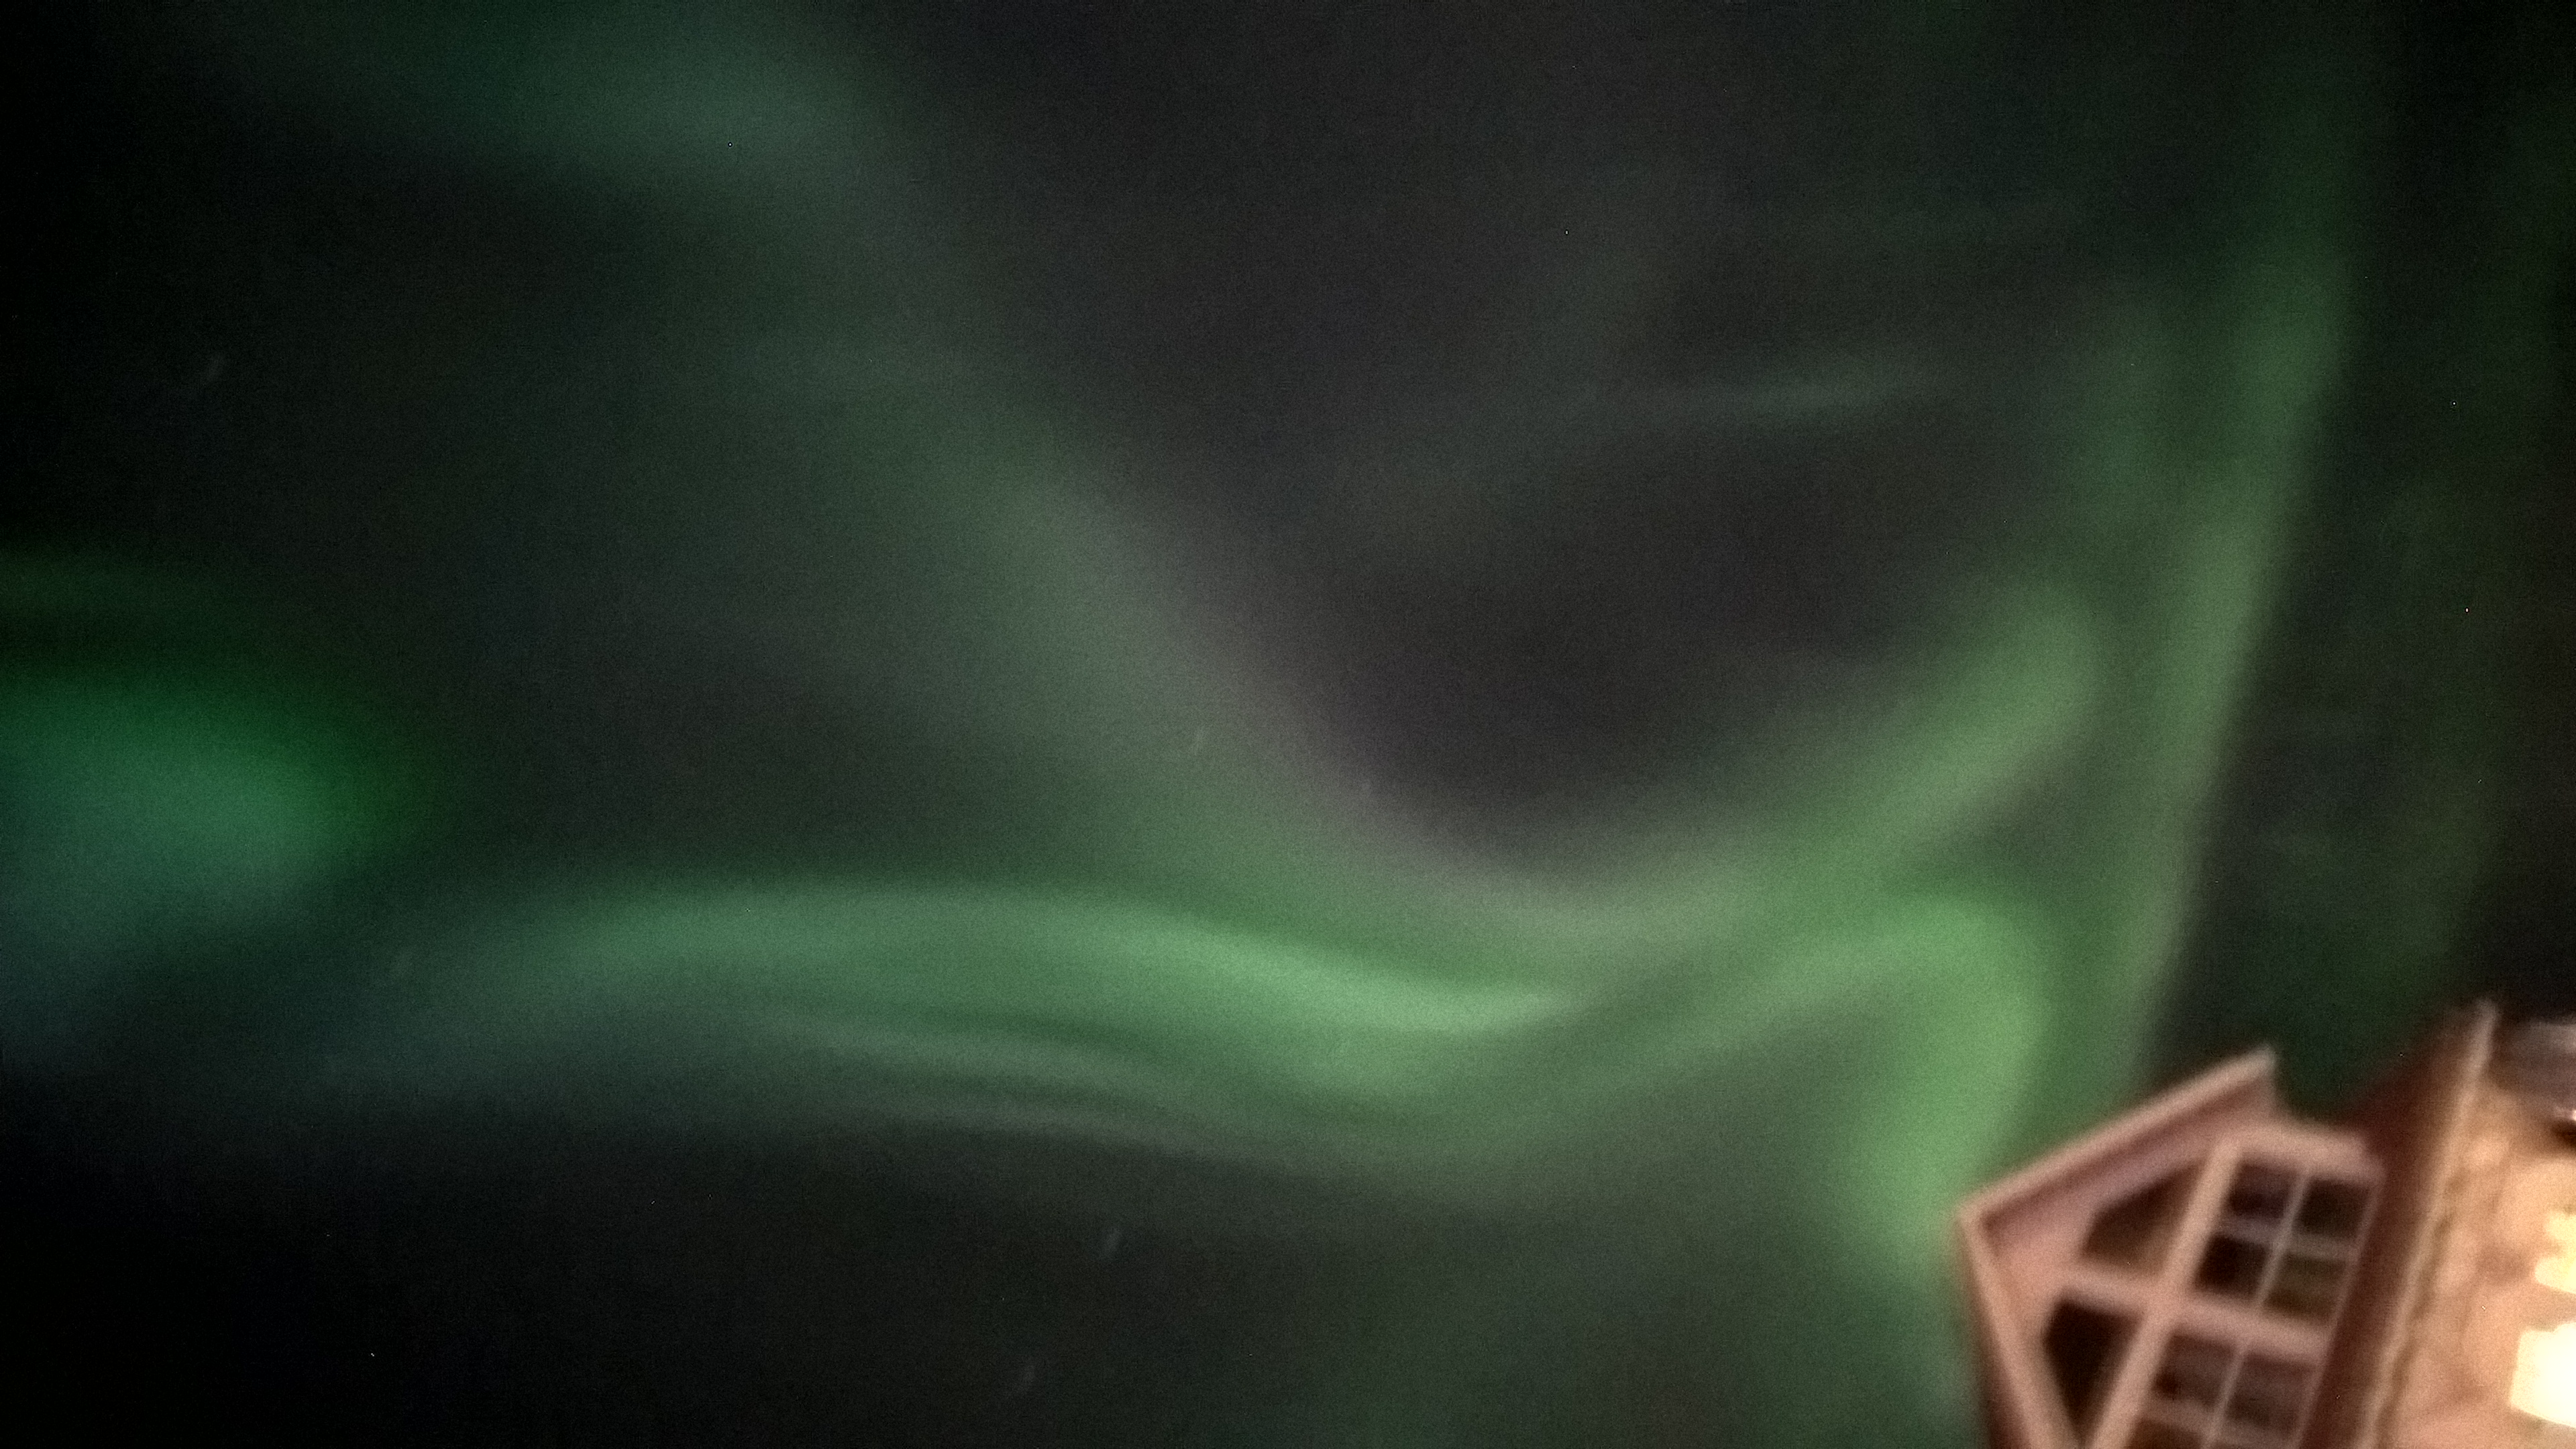
\includegraphics[width=90mm]{northernlights.jpg}
\caption{Bilde av nordlys tatt i Andenes \label{overflow}}
\end{figure}

N{\aa}r vi kom tilbake til ASC, valge de fleste av oss {\aa} g{\aa} til stranda nedenfor romsenteret for {\aa} se p{\aa} nordlyset. Ettersom denne stranda l{\aa} skjermet for lyset rundt, var det lettere {\aa} se nordlys, og det dukket opp en nordlysoval p{\aa} himmelen.

\begin{figure}[H]
\centering
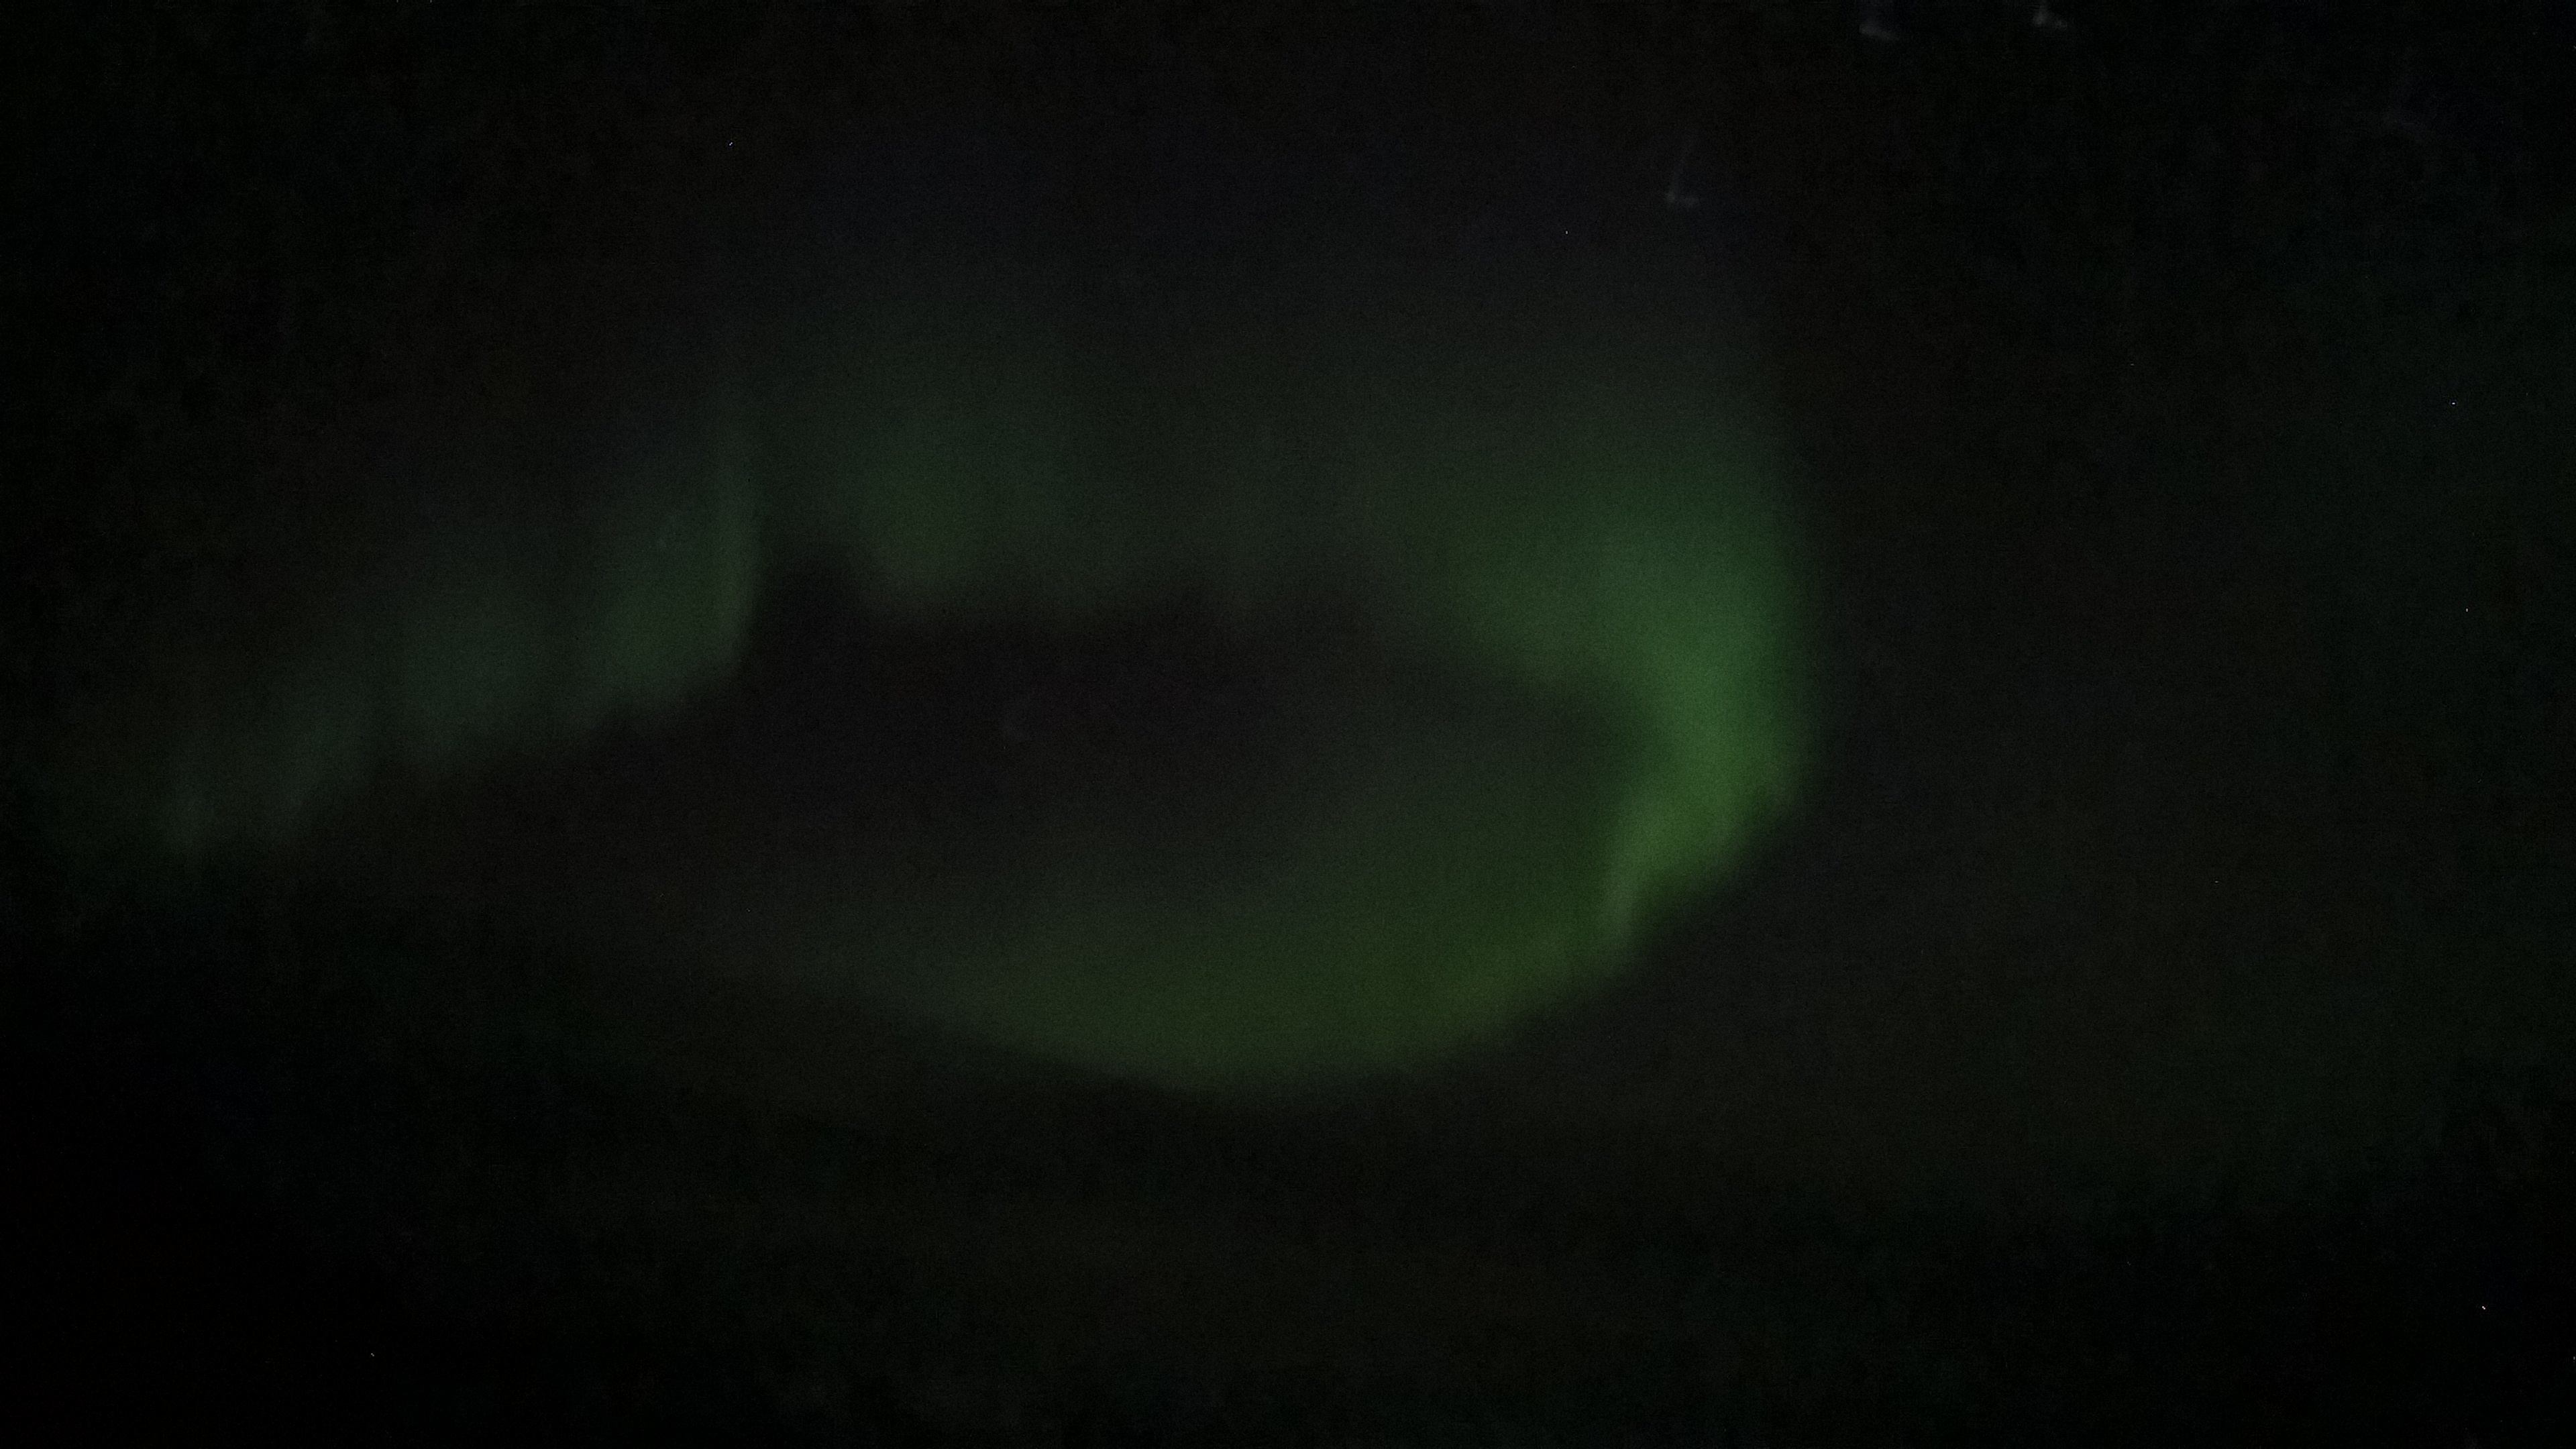
\includegraphics[width=90mm]{lightoval.jpg}
\caption{Bilde av nordlys tatt fra stranda nedenfor ASC \label{overflow}}
\end{figure}

\section*{Dag 3 - Onsdag 5/10}
P{\aa} onsdagen startet vi med en forelesning om aktivitetene rundt 4DSPACE ved UiO, f{\o}r vi gikk tilbake til gruppejobbingen. Vi fortsatte med {\aa} sette sammen modellrakettene. Vi fikk ogs{\aa} dataene fra v{\ae}rballongen, som hadde n{\aa}dd en h{\o}yde p{\aa} 26 km, f{\o}r den hadde bristet. Ved hjelp av MATLAB og Google Earth fikk vi visualisert dataene, slik at vi s{\aa} hvordan sidevinden, luftfuktigheten etc.. varierte med h{\o}yden. Utp{\aa} ettermiddagen hadde vi forelesning om hvordan man launcher raketter, f{\o}r vi igjen gikk tilbake til klasserommet og jobbet med modellrakettene. Planen var at vi skulle skyte opp modellrakettene v{\aa}re denne dagen, men p{\aa} grunn av mye vind ble vi n{\o}dt til {\aa} utsette det. 

\begin{figure}[H]
\centering
\begin{subfigure}{.5\textwidth}
  \centering
  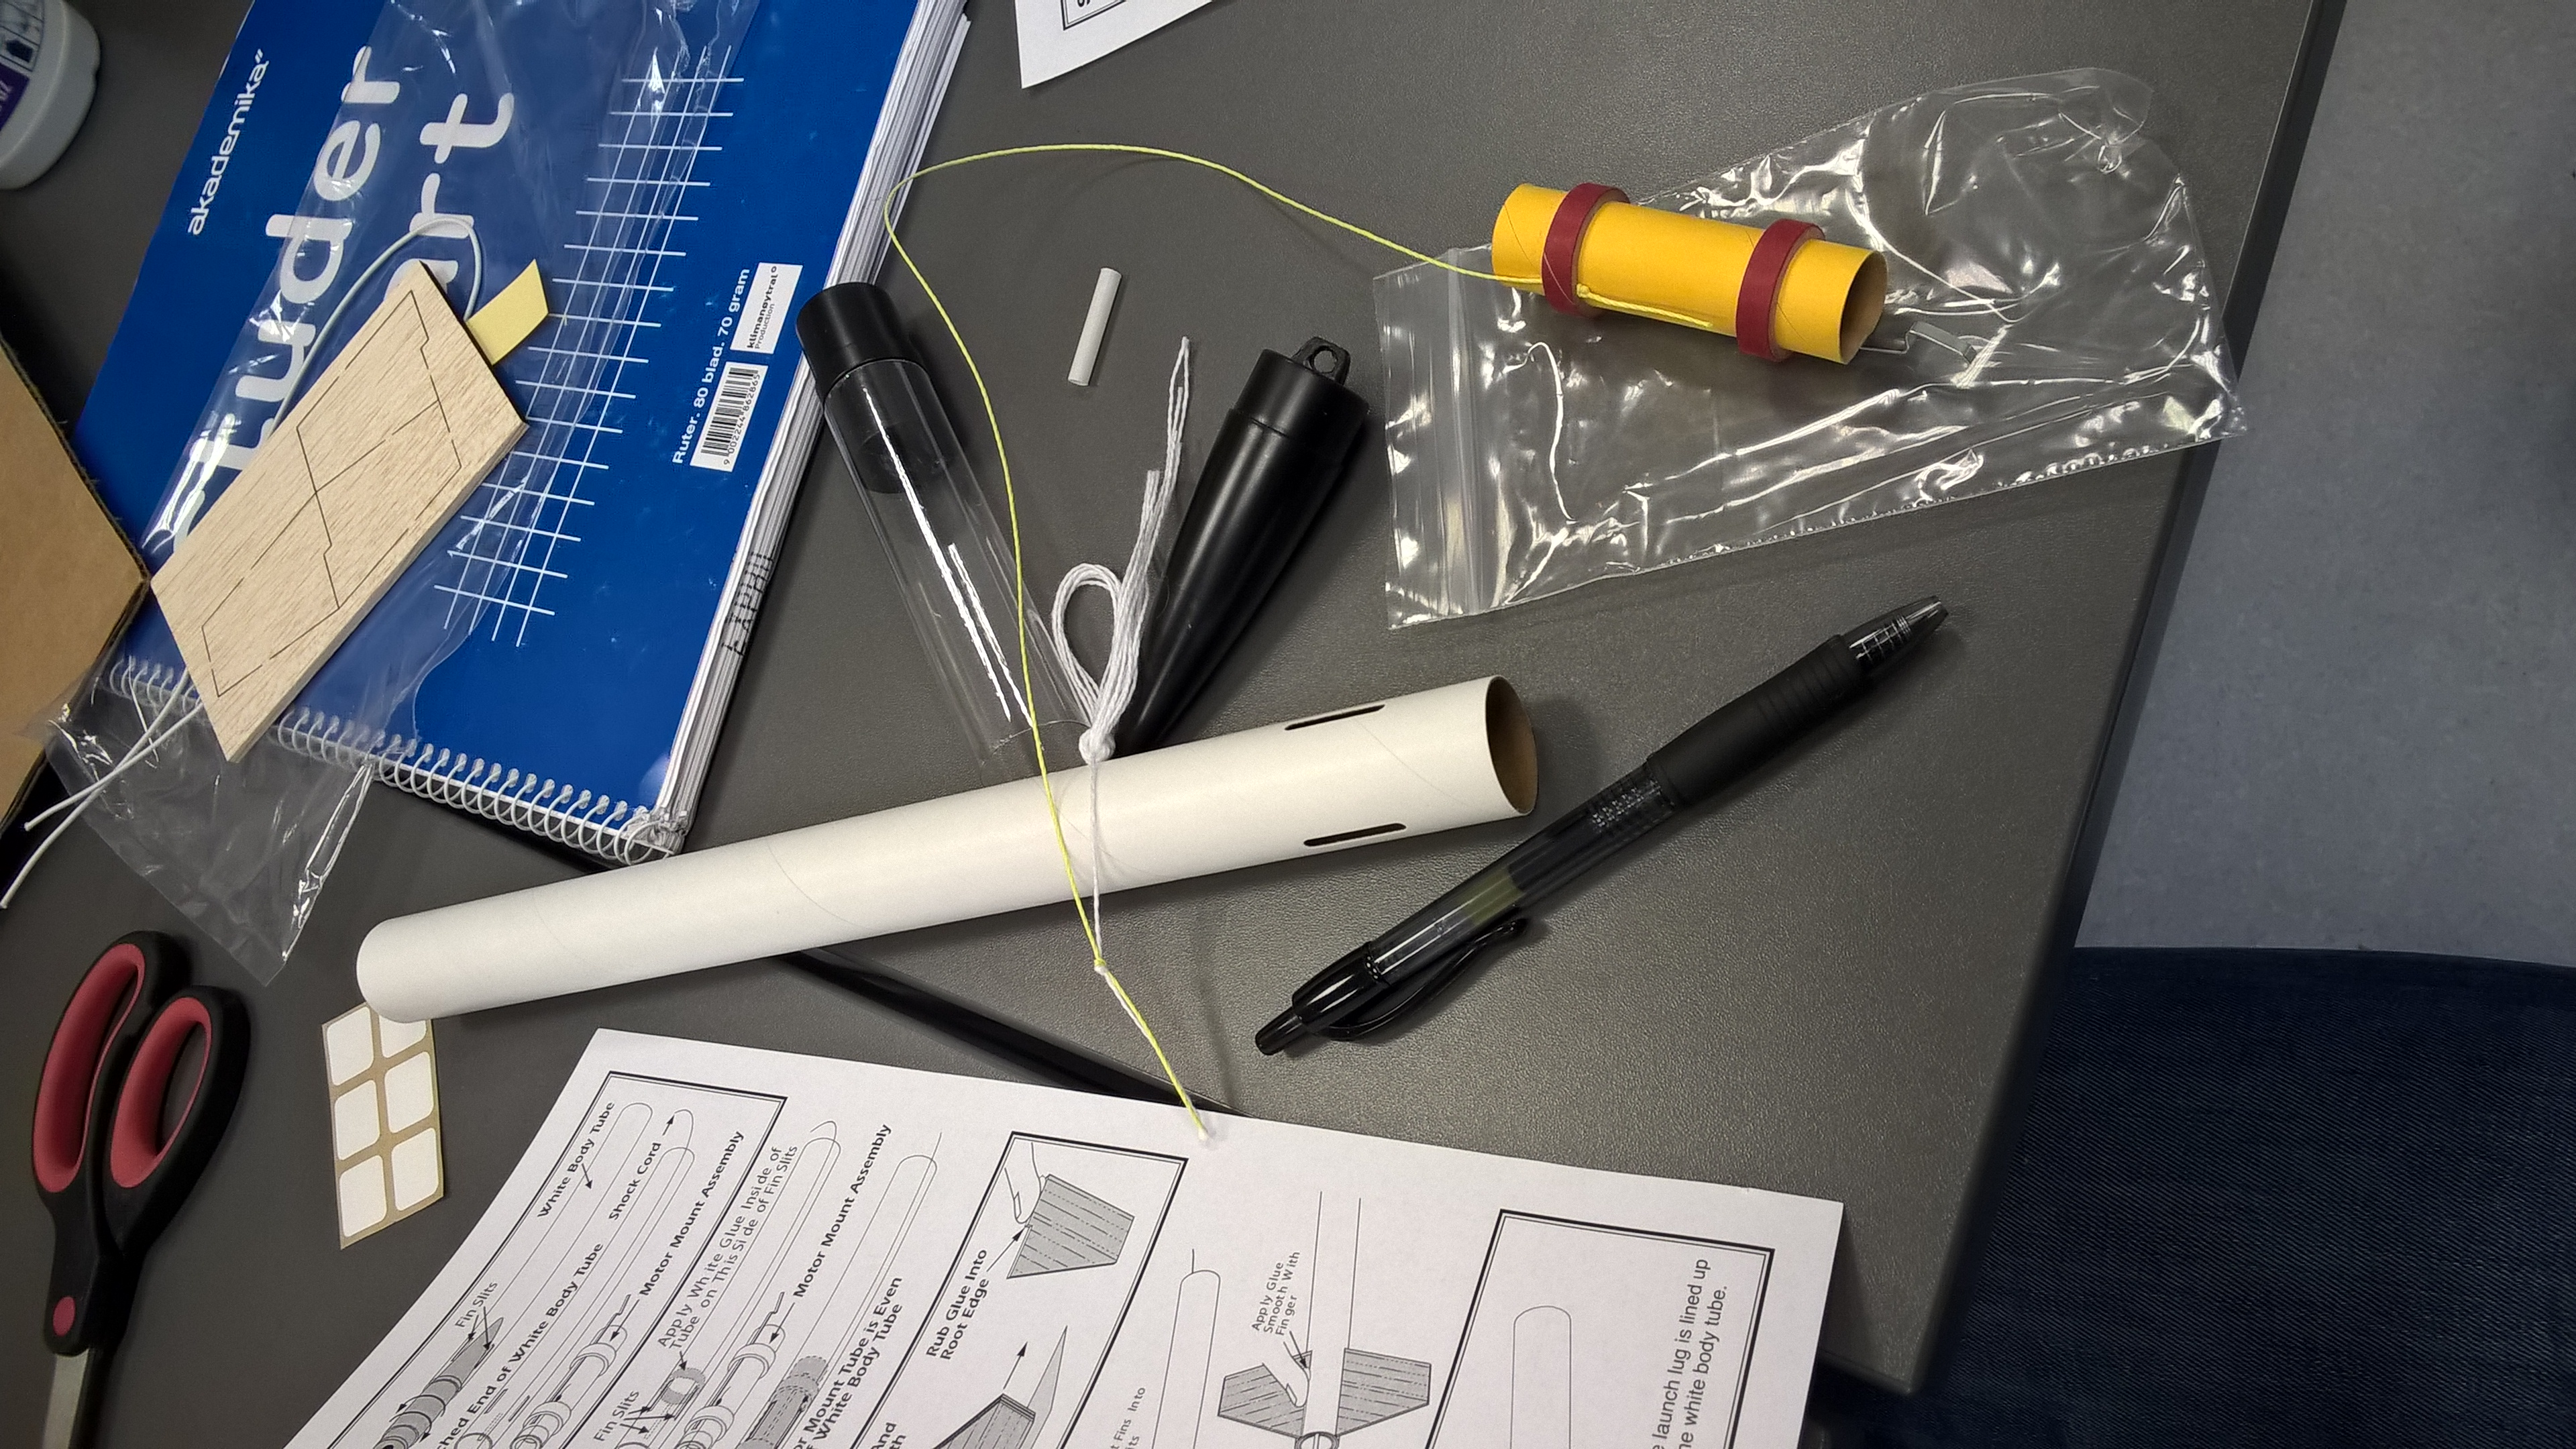
\includegraphics[width=90mm]{modelrocket1.jpg}
  \caption{Under byggingen av modellraketten.}
  \label{fig:sub1}
\end{subfigure}
\begin{subfigure}{.5\textwidth}
  \centering
  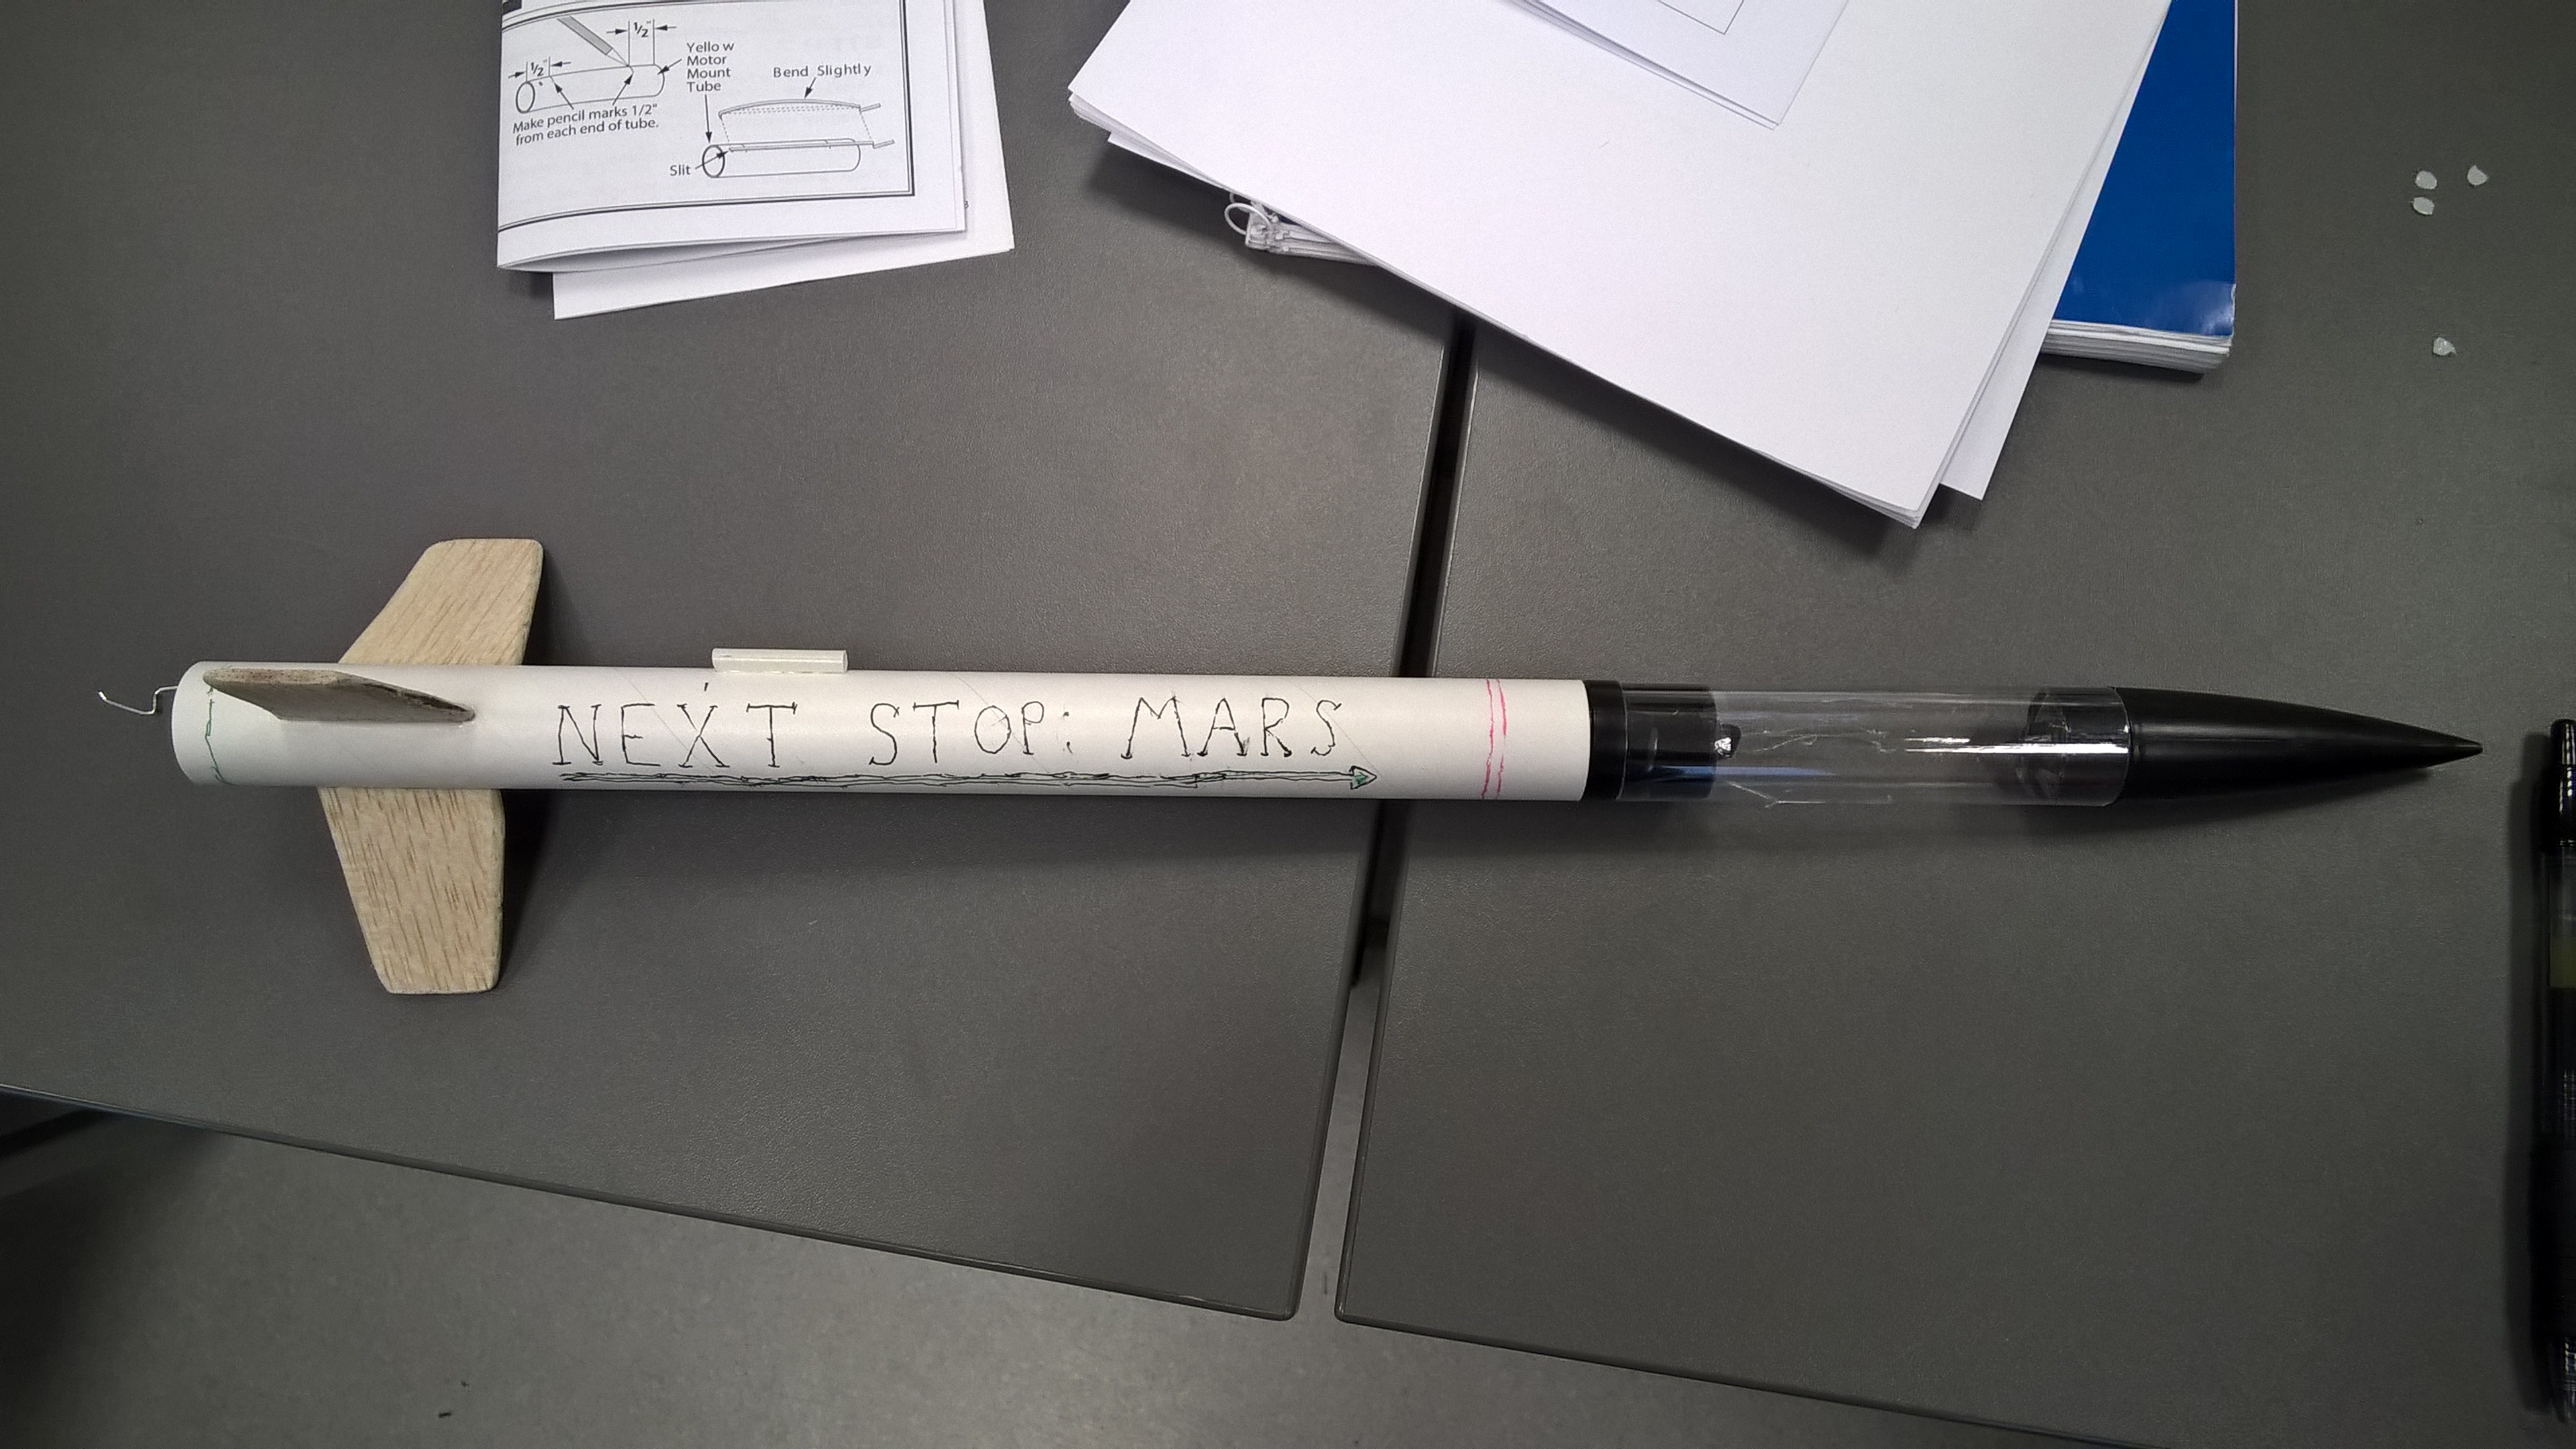
\includegraphics[width=90mm]{modelrocket2.jpg}
  \caption{Ferdig modellrakett som skal til Mars.}
  \label{fig:sub2}
\end{subfigure}
\caption{Bilder av modellraketten}
\label{fig:test}
\end{figure}

Etter vi hadde blitt ferdig med byggingen av modellrakett, var det klart for photoshoot ikledd NASA-drakter. 

\begin{figure}[H]
\centering
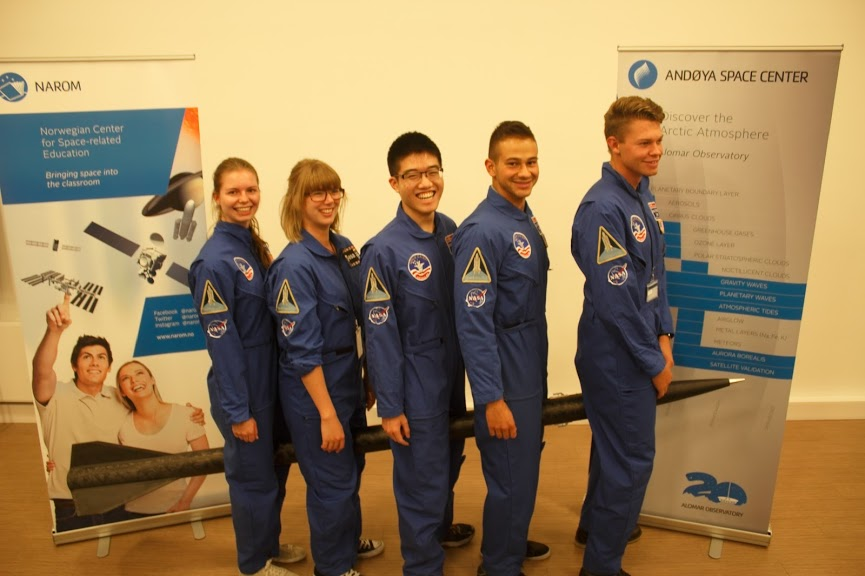
\includegraphics[width=90mm]{photoshoot.jpg}
\caption{Photoshoot ikledd NASA-drakter. Fra venstre: Dorthea Gjestvang, Nina Kristine Eriksen, Henry Su, David Bellerose og Even Marius Nordhagen (meg). Bildet er tatt av Gabriel Sigurd Cabrera. \label{overflow}}
\end{figure}

Senere p{\aa} kvelden spilte vi biljard og bordtennis, noe som ikke var en uvanlig aktivitet under oppholdet p{\aa} ASC. 

\section*{Dag 4 - Torsdag 6/10}
Det var dagen for oppskyting av raketten vi hadde jobbet s{\aa} mye med. P{\aa} morgenen hadde gruppe A og C hver sin korte presentasjon hvor de forklarte hvordan ting sto til f{\o}r raketten skulle launches, f{\o}r det var klart for en "f{\o}roppskytningssamtale" med sikkerhetsinstruksjoner. P{\aa} dette m{\o}tet ble vi ogs{\aa} enige om navnet til raketten, som endte med {\aa} v{\ae}re Rocket McRocketface, forkortet RMR7. Under selve rakettoperasjonen satt jeg og gruppa mi p{\aa} Science Center, hvor vi i teorien skulle studere vindkartet og si ifra n{\aa}r det passet best {\aa} sende opp raketten, men i praksis var vi nok ikke s{\ae}rlig viktige. Rakettoppskytningen gikk som forventet, noe de ogs{\aa} konkluderte med p{\aa} "etteroppskytningssamtalen". 

Litt f{\o}r p{\aa} dagen hadde noen ansatte sendt opp en ny v{\ae}rballong (som inneholdt Hydrogengass), for {\aa} ha et overblikk over hvordan vinden var h{\o}yere opp i atmosf{\ae}ren. N{\aa}r vi skulle forberede presentasjonen, baserte vi oss blandet annet p{\aa} dataene fra denne ballongen. Vi holdt p{\aa} med denne forberedelsen til ganske langt utp{\aa} kvelden, mens en annen gruppe gikk p{\aa} butikken for {\aa} kj{\o}pe {\o}l. Etter {\aa} ha fullf{\o}rt presentasjonen, gikk noen av oss for {\aa} bade i sj{\o}en, noe vi fikk diplom for senere. Veien var kort til badstuen etter badet. Etter dette besto kvelden av {\o}l og to bursdagsbarn n{\aa}r klokka passerte 12. Vi feiret med kortspill og sjakk, f{\o}r vi ble jaget til sengs klokka ett. 

\begin{figure}[H]
\centering
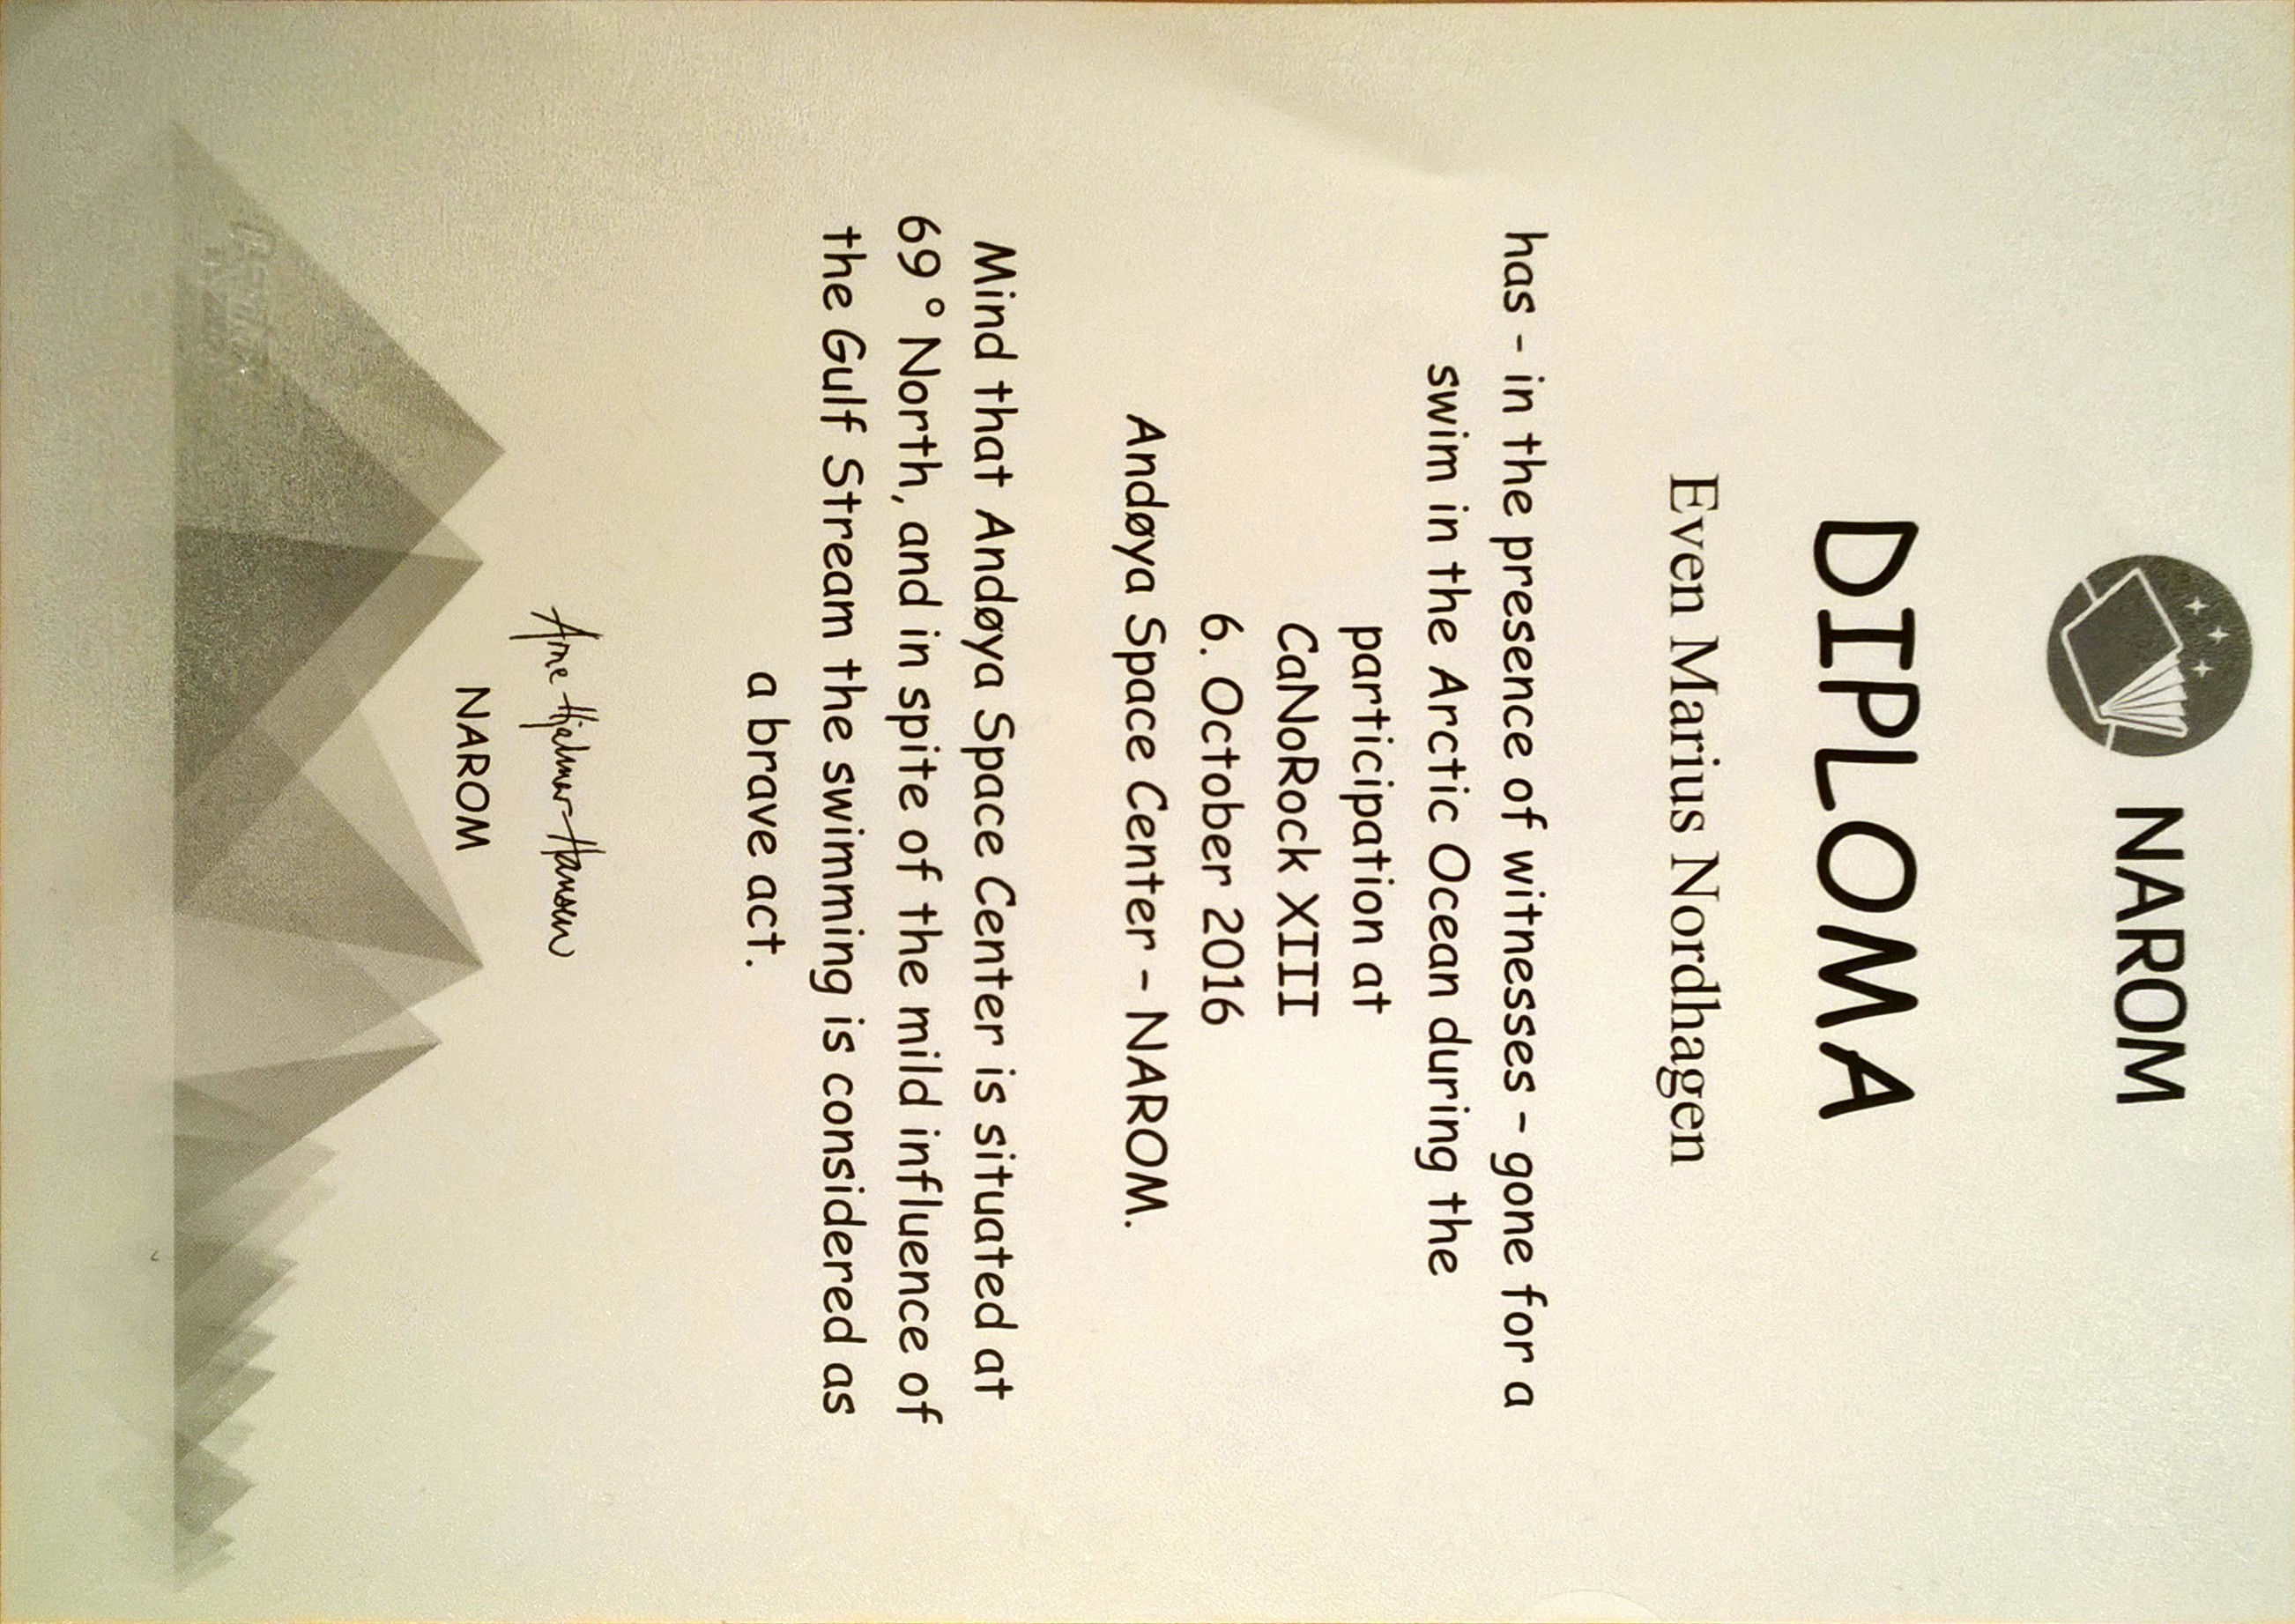
\includegraphics[width=90mm]{Diploma.jpg}
\caption{Diplom for {\aa} ha badet i nordsj{\o}en. \label{overflow}}
\end{figure}
\begin{figure}[H]
\centering
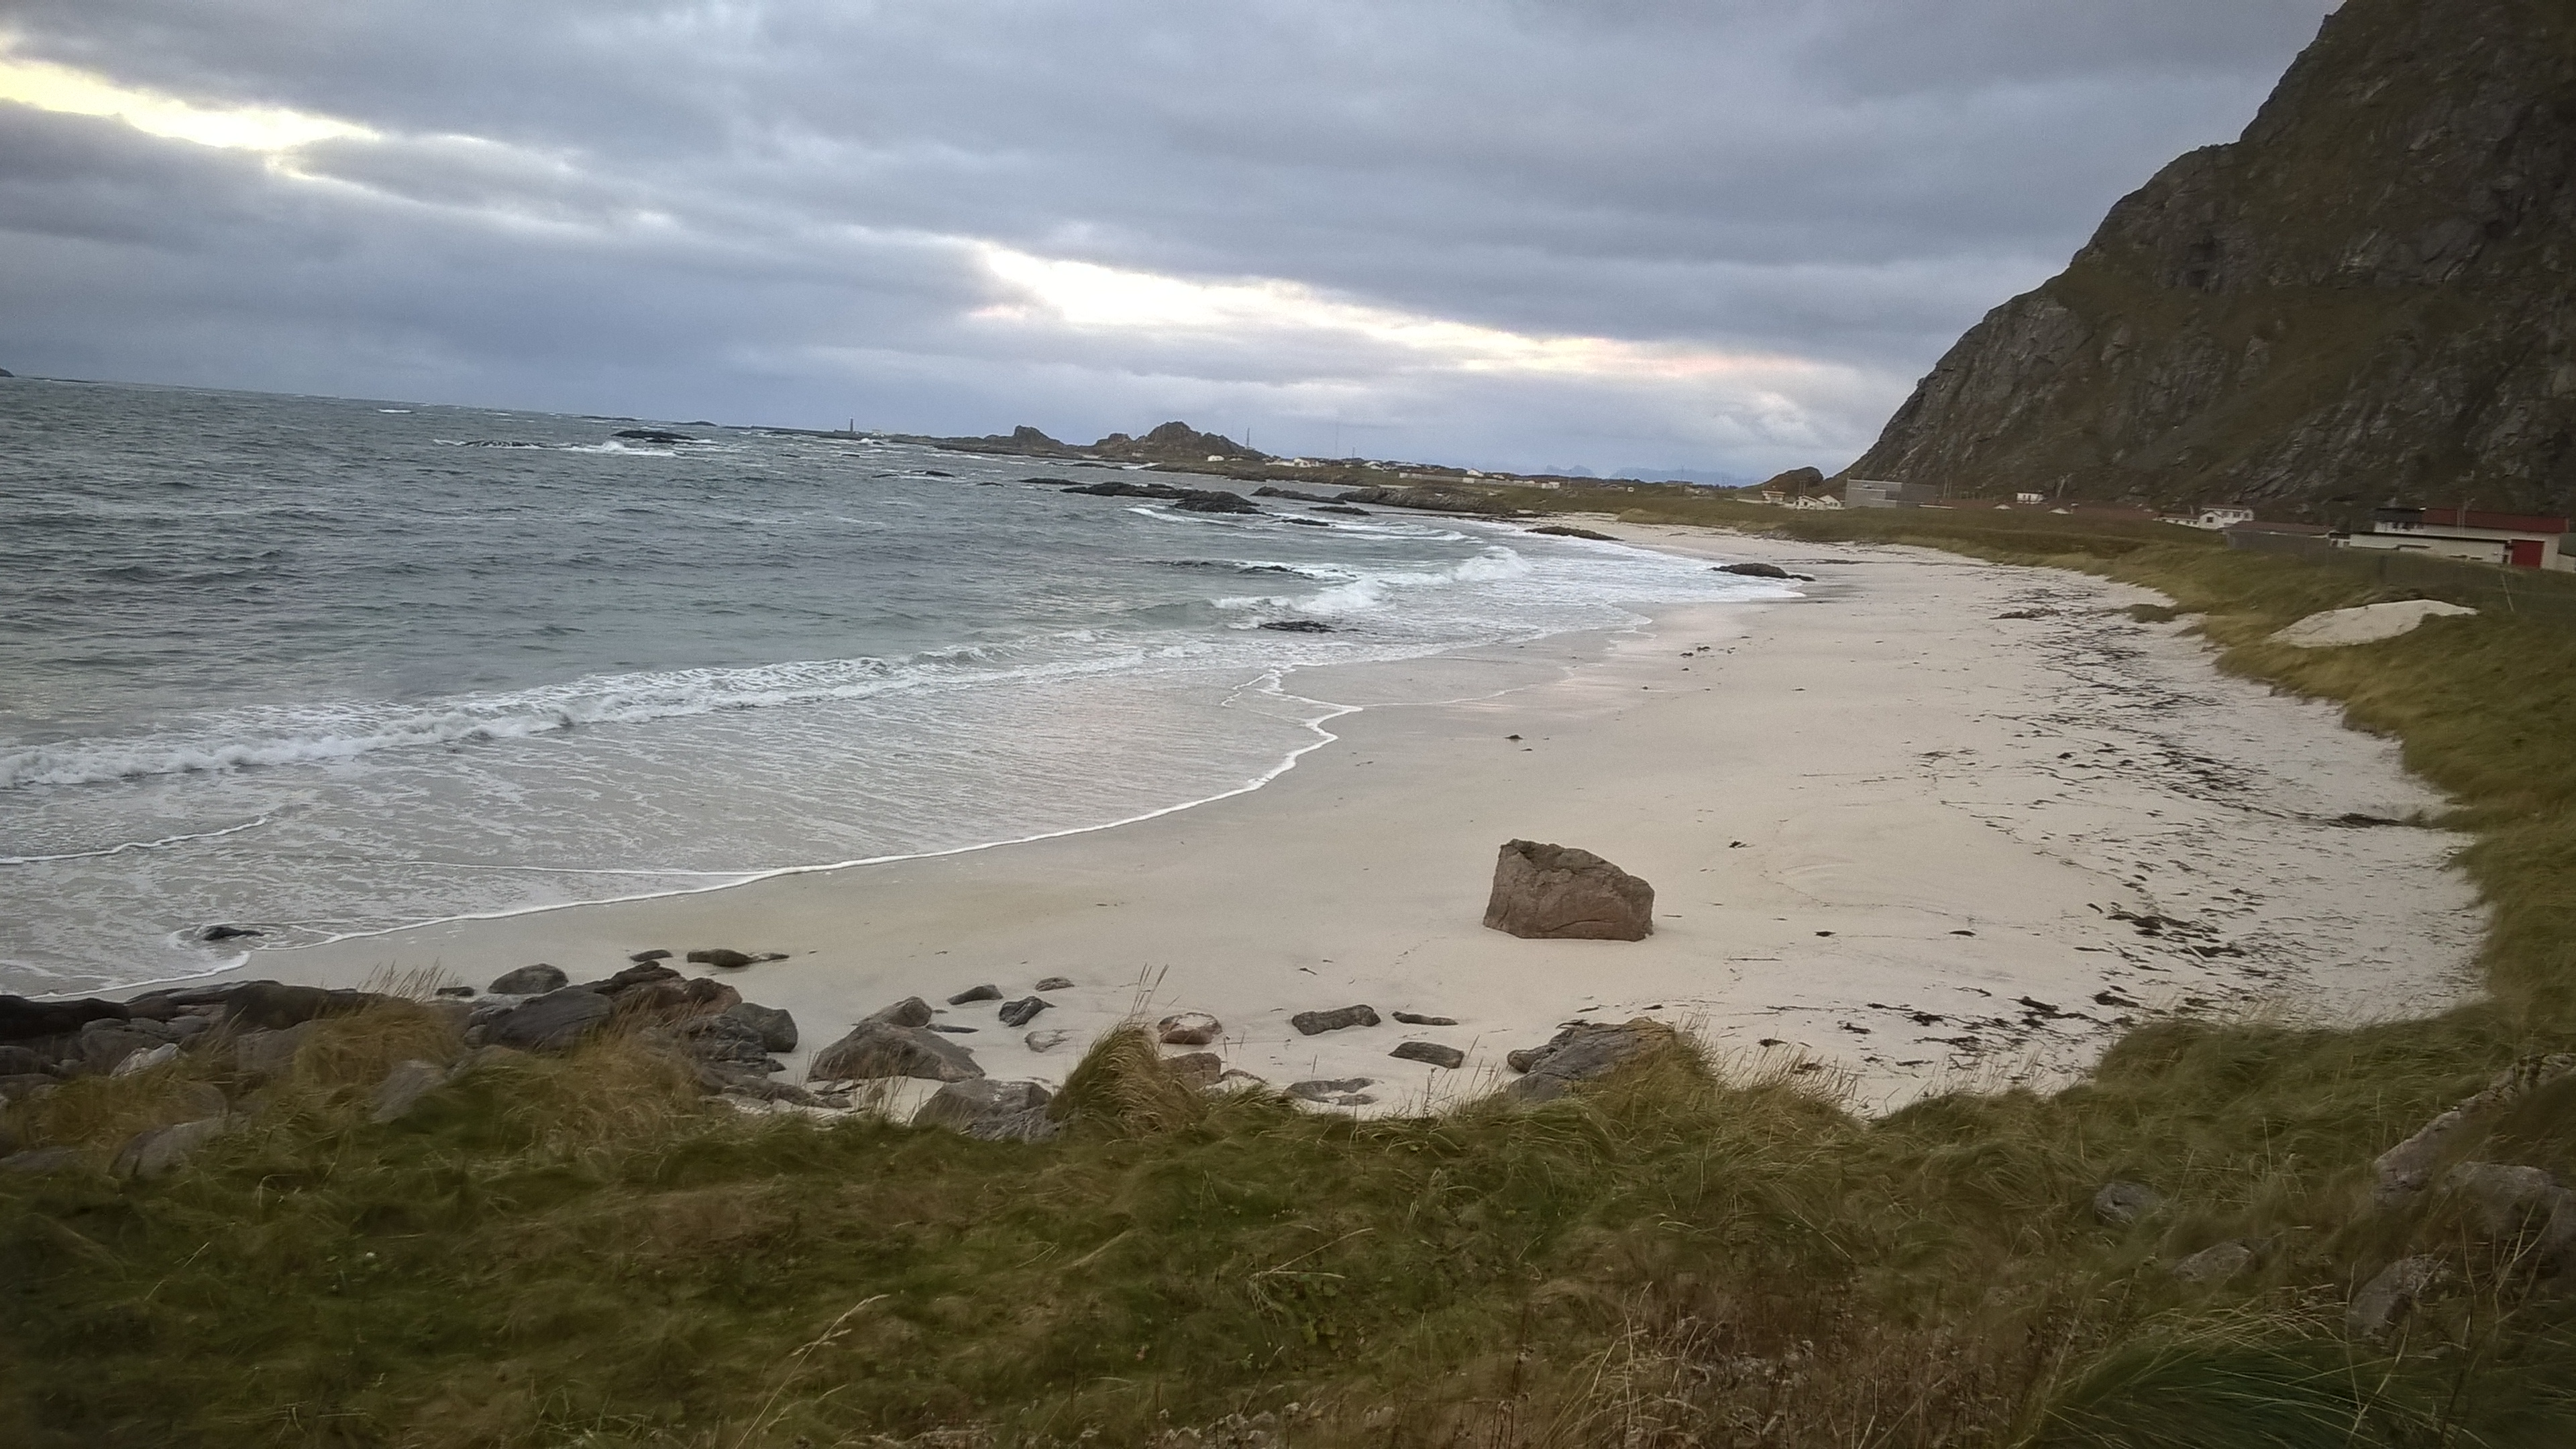
\includegraphics[width=90mm]{strand.jpg}
\caption{Stranden vi badet p{\aa}. Minnet om syden helt til vi kjente p{\aa} vannet. \label{overflow}}
\end{figure}


\section*{Dag 5 - Fredag 7/10}
Fredagen startet med utsjekking fra hostellet, f{\o}r vi tok minibuss til ALOMAR. Her fikk vi en innf{\o}ring i hvordan instrumentene fungerer, med vekt p{\aa} LADARene. Deretter var det omvisning rundt p{\aa} bygget, hvor vi blant annet fikk se de mobile LADARene.

\begin{figure}[H]
\centering
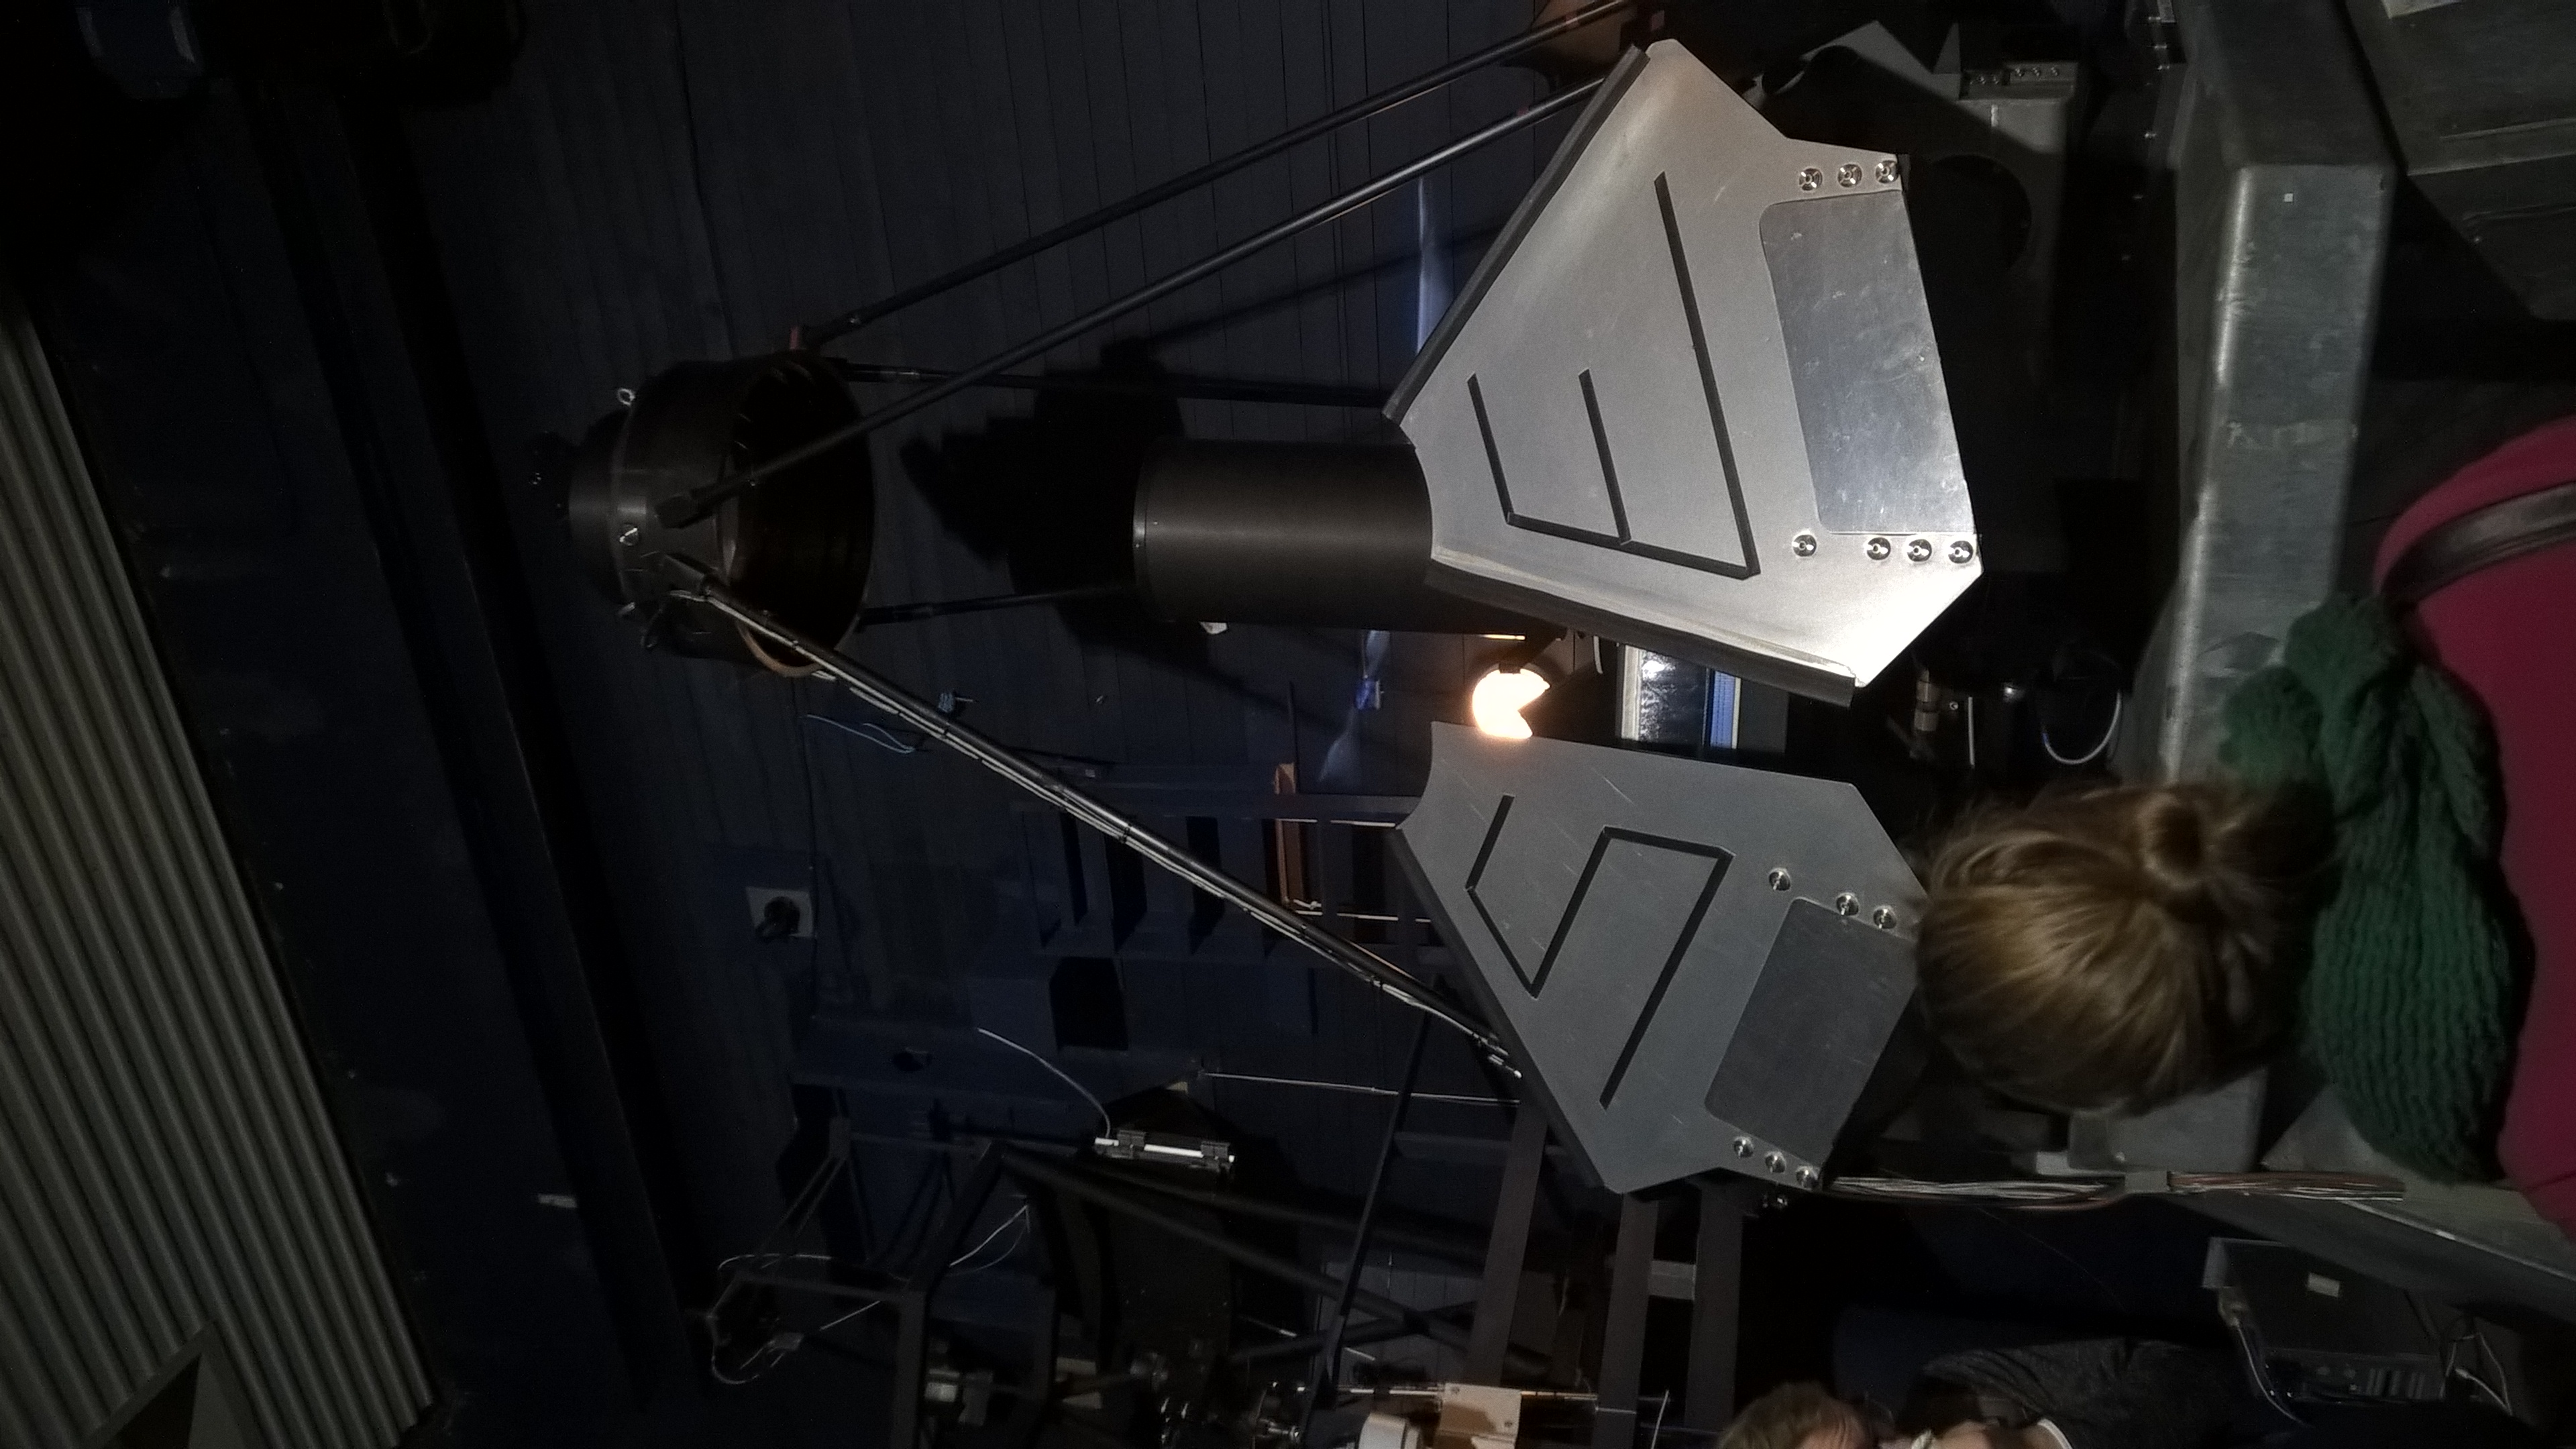
\includegraphics[width=90mm]{ladar.jpg}
\caption{Mobil LADAR p{\aa} ALOMAR. \label{overflow}}
\end{figure}

Deretter bar det ned igjen mot ASC, nedover ganske bratte veier. P{\aa} turen oppover kunne vi ikke fylle minibussene fulle i frykt for {\aa} ikke komme opp. 

\begin{figure}[H]
\centering
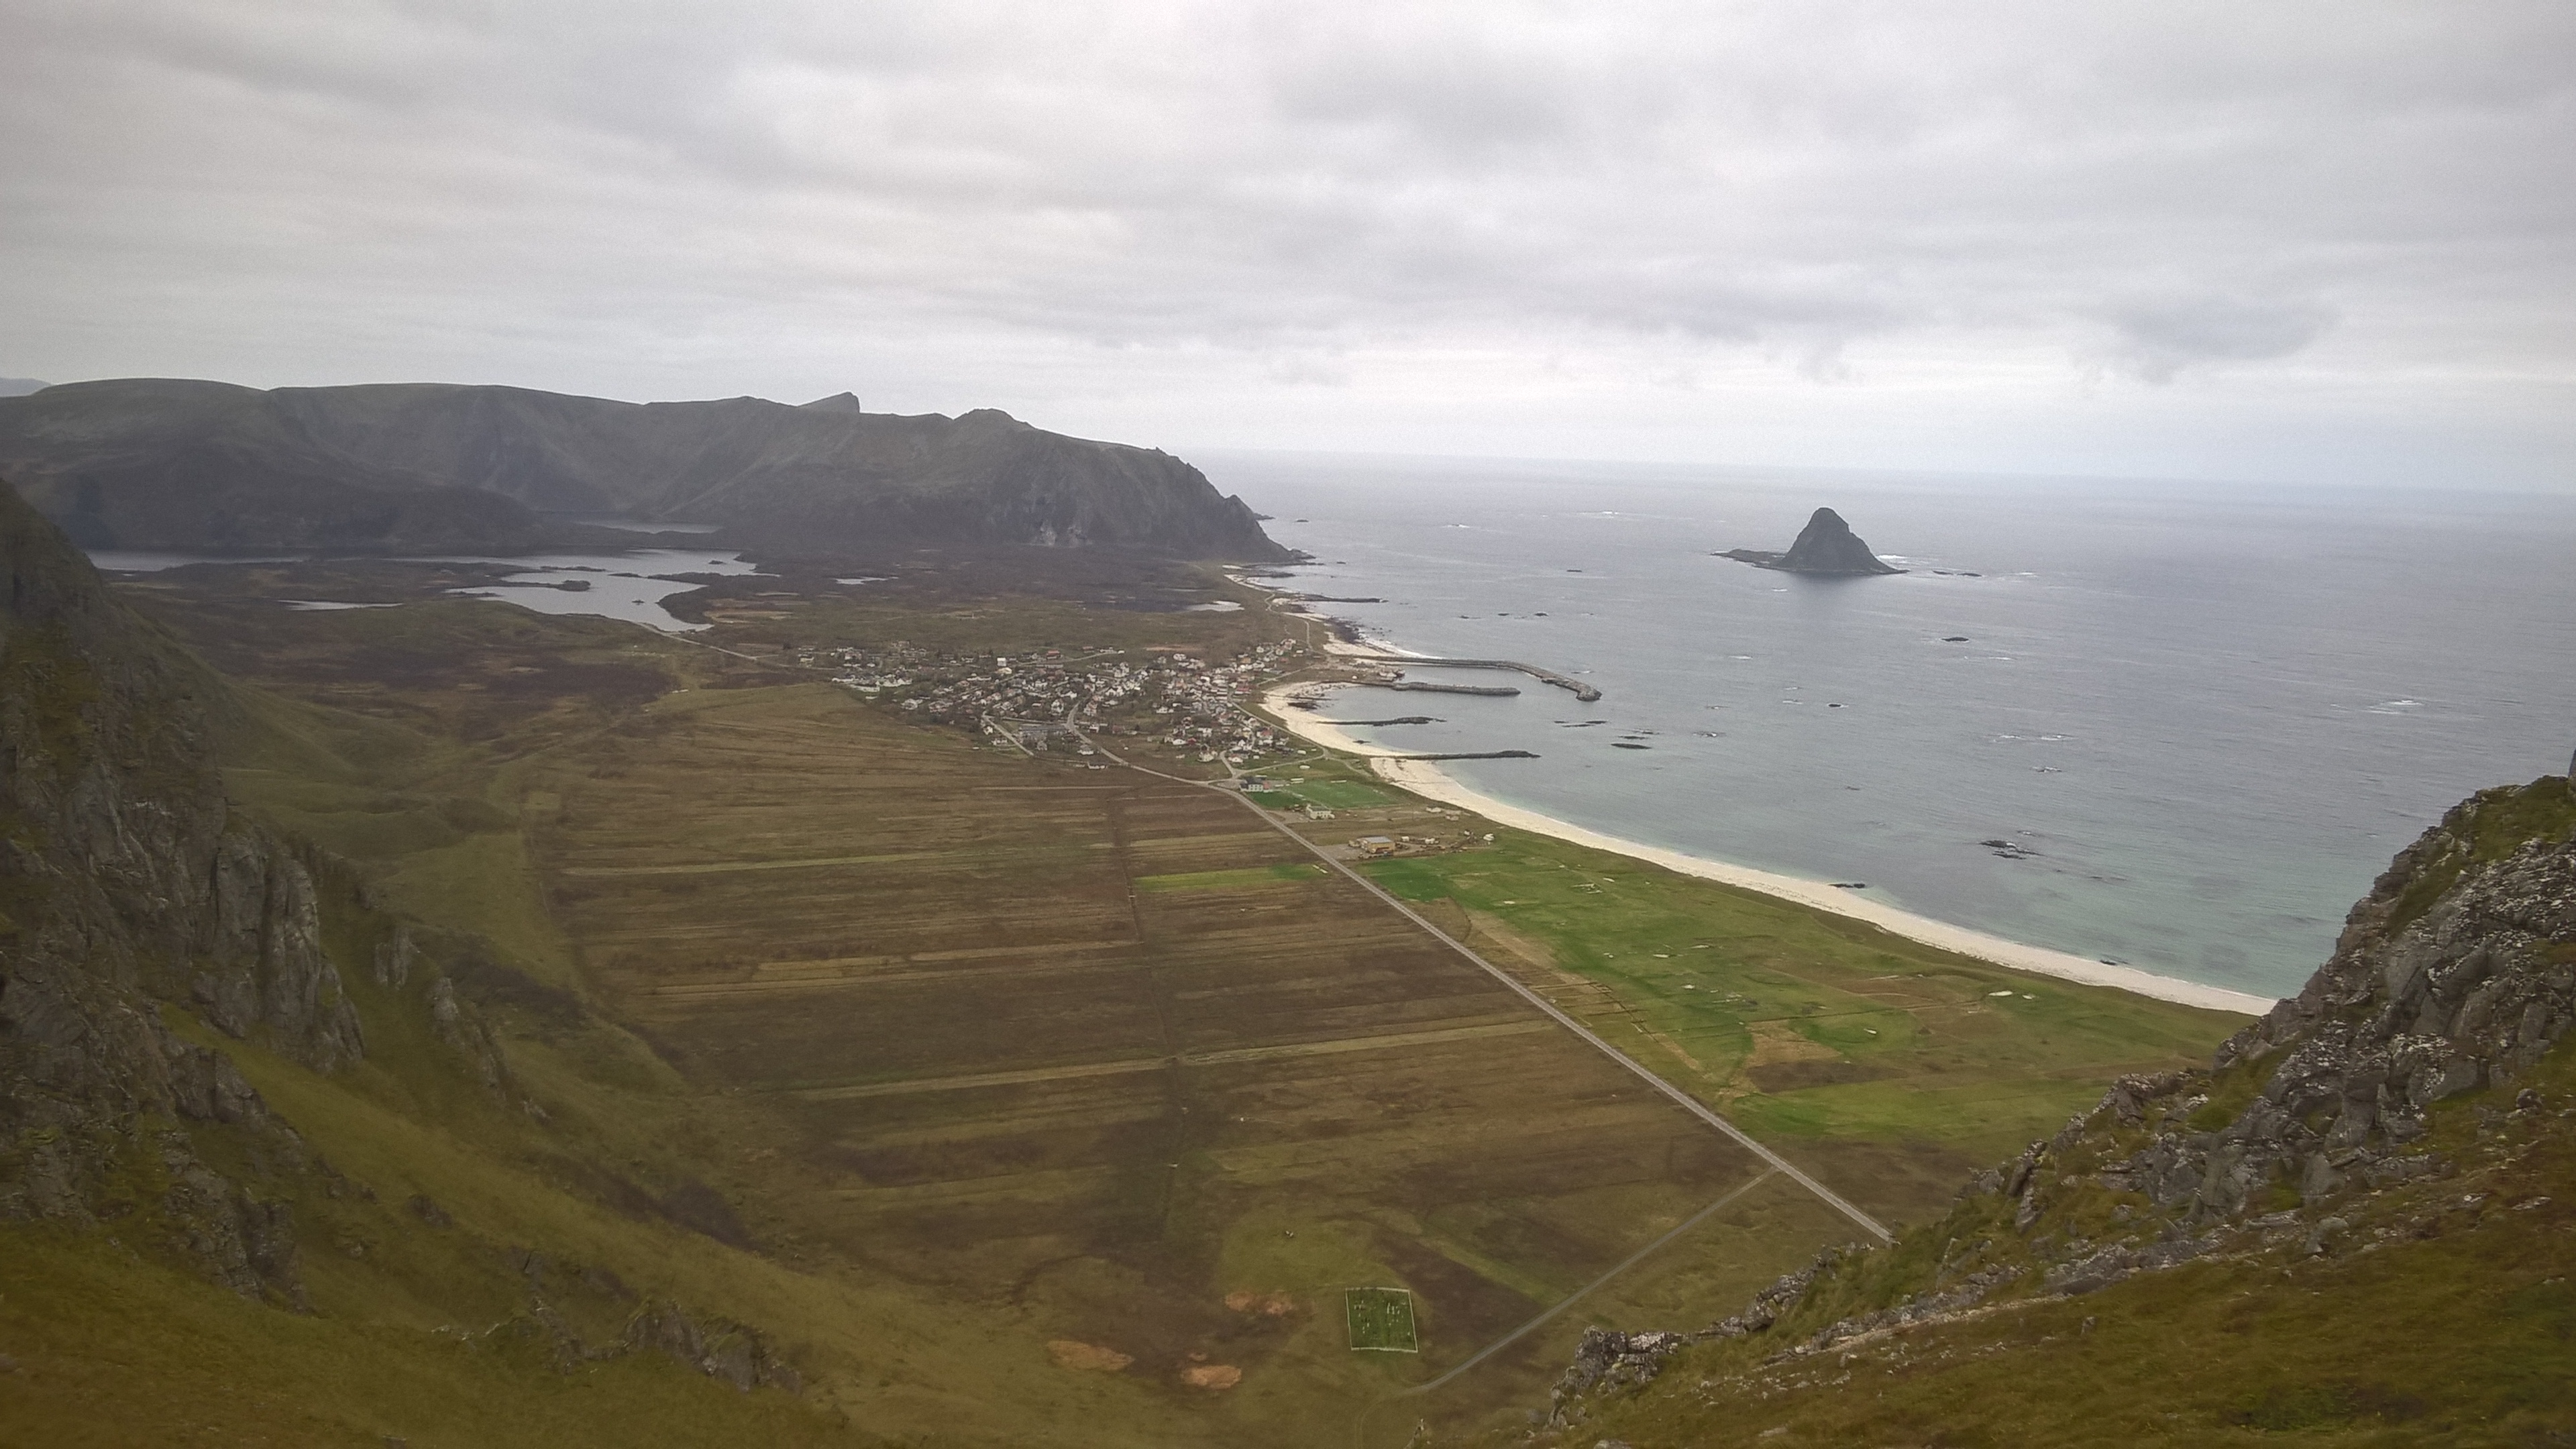
\includegraphics[width=90mm]{view.jpg}
\caption{Utsikt fra veien opp mot ALOMAR. \label{overflow}}
\end{figure}

Deretter var det klart for presentsjoner, og vi var siste gruppe ut. Vi presenterte simuleringen v{\aa}r av raketten, som bare varte i 0.002 sekunder, dataene fra ballongen og litt om prinsippet bak ballongene. Vi avsluttet CaNoRock 13 med kake, f{\o}r vi dro til Andenes og tok fly sammen til Troms{\o}. 

\section*{Mat}
Noe jeg ikke har nevnt noe s{\ae}rlig om under referatet er maten, noe jeg synes passer best under en egen seksjon. Hver dag har vi f{\aa}tt servert frokost, et fruktm{\aa}ltid, lunsj middag og kveldsmat. Frokost og kveldsmat har stort sett v{\ae}rt br{\o}dmat, mens vi har f{\aa}tt nye lunsj- og middagretter hver dag. Lunsjen varierte fra karbonader med egg, til tomatsuppe, mens vi fikk alt fra italiensk og asiatisk til meksikansk til middag. Siste lunsjen var komponert av restene fra hele uka.
\end{document}